\documentclass{article}
\usepackage{graphicx} % Required for inserting images
\usepackage{sidecap}
\usepackage{wrapfig}
\usepackage[utf8]{inputenc} %lettere accentate da tastiera 
\usepackage[T1]{fontenc} % higher quality font encoding
\usepackage{lipsum}
\usepackage{subfigure}% per mettere immagini vicine 
%load the font and set it to default
\usepackage{amsmath,amsthm,amsfonts}
\usepackage[english,italian]{babel}
\usepackage{amsmath}
\usepackage{pgfplots}
\usepackage{url}
\pgfplotsset{compat=1.18}
\usepackage{geometry}
\geometry{a4paper,top=3cm,bottom=3cm,left=3.5cm,right=3.5cm,%
	heightrounded,bindingoffset=5mm}
\usepackage{tikz}
\usepackage[x11names]{xcolor}
\usepackage{tcolorbox}
\tcbuselibrary{theorems}
\usepackage{cancel}

\usepackage{hyperref}
\hypersetup{
	colorlinks=false,
	linkcolor=blue,
	filecolor=magenta,      
	urlcolor=blue,
	pdftitle={Analisi II},
	pdfpagemode=FullScreen,
}
\usepackage{enumitem}

\newtheorem{teorema}{Teorema}[subsection]
\theoremstyle{definition}
\newtheorem*{definizione}{Definizione}
\newtheorem*{proprieta}{Proprietà}
\newtheorem*{corollario}{Corollario}
\newtheorem*{formula}{Formula}
\newtheorem*{proposizione}{Proposizione}
\newtheorem{prop}{Proposizione}
\newtheorem*{lemma}{Lemma}

\newtheorem{nulla}{}
\newtcbtheorem[number within=section]{teo}{}{colback=black!5 ,colframe=black!90,nameref/.style={}}{}
\newcommand{\R}{\mathbb{R}}
\newcommand{\D}{\mathbb{D}}
\newcommand{\V}{\mathbb{V}}
\newcommand{\K}{\mathbb{K}}
\newcommand{\w}{\mathbb{W}}
\newcommand{\C}{\mathbb{C}}
\newcommand{\norma}{||\cdot||}
\newcommand{\Rn}{\R^n}
\newcommand{\la}{\lambda}
\newcommand{\on}{^{\perp}}
\newcommand{\A}{\mathbb{A}}
\newcommand{\xb}{\overline{x}}
\newcommand{\fn}{f: A\subseteq \Rn \rightarrow \R}
\newcommand{\fnn}{f: A\subseteq \Rn \rightarrow \Rn}
\newcommand{\fnm}{f: A\subseteq \Rn \rightarrow \R^m}
\newcommand{\s}{$\Sigma$}
\newcommand{\abs}[1]{|#1|}


\title{Elettrotecnica }
\author{Luca Mombelli}
\date{2024-25}

\begin{document}
	\maketitle
		\tableofcontents
	\newpage
	\section{Circuiti in DC}
\begin{teo*}{Legge di Kirchhoff per le correnti (KCL)}
	In un nodo la somma delle correnti entranti ( assunte positive ) e uscenti (assunte negative) è nulla
	\begin{equation}
    \sum_{i=1}^n I_i = 0
    \end{equation}
\end{teo*}
\begin{teo*}{Legge di Kirchhoff per le differenze di potenziale (KVL)}
	In una maglia la somma algebrica delle tensioni è nulla 
	\begin{equation}
    \sum_{i=1}^n V_i = 0
    \end{equation}
\end{teo*}
Ponte di Wheastone 
\begin{figure}[h]
	\centering
	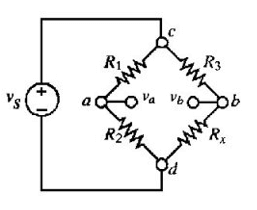
\includegraphics[scale=0.40]{immagini/ponte}
	\caption{}
	\label{fig:ponte-di-wheatstone-500x400}
\end{figure}
$$R_4=\frac{R_2 \times R_3}{R_1}$$ ottenuta con il ponte in equilibrio quindi con $v_{ab}=0$
Inoltre la differenza di potenziale tra i due capi si può calcolare come 
$$v_{ab}=v_{ad}-v_{bd}=E\left( \frac{R_2}{R_1+R_2}-\frac{R_x}{R_3+R_x}\right) $$
\begin{teo*}{Teorema del generatore equivalente }
	\begin{itemize}
		\item Thevenin : \\
		Un circuito resistivo lineare , ai fini del suo comportamento ad una qualsiasi coppia di terminali a e b ,  è equivalente ad un generatore ideale di tensione in serie ad un resistore. La tensione $v_T$ del generatore è la tensione che si ha tra i terminali , quando sono aperti. La resistenza $R_T$ del resistore è la resistenza equivalente vista dai terminali   con i generatori indipendenti spenti 
		\begin{center}
			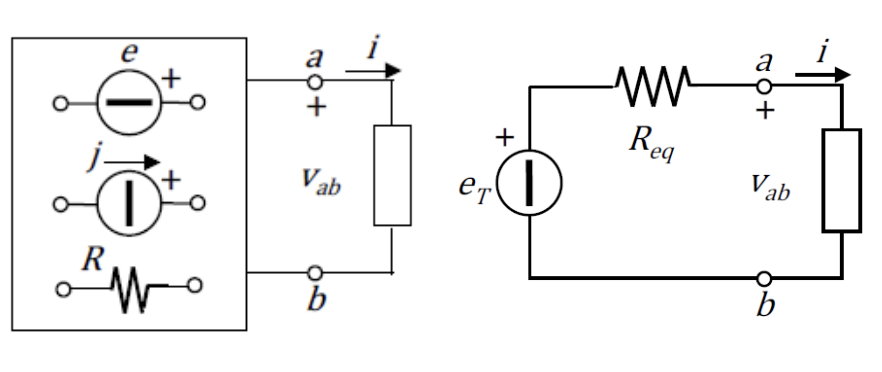
\includegraphics[scale=0.40]{immagini/th}
		\end{center}
		\item Norton :\\
		 Un circuito resistivo lineare , ai fini del suo comportamento ad una qualsiasi coppia di terminali a e b ,  è equivalente ad un generatore ideale di corrente in parallelo ad un resistore. La corrente $I_N$ del generatore è la corrente che scorre nei terminali quando questi sono in corto circuito ( corrente di cc).La Resistenza $R_N$ del resistore è la resistenza equivalente al circuito con i generatori indipendenti spenti	
		\begin{center}
			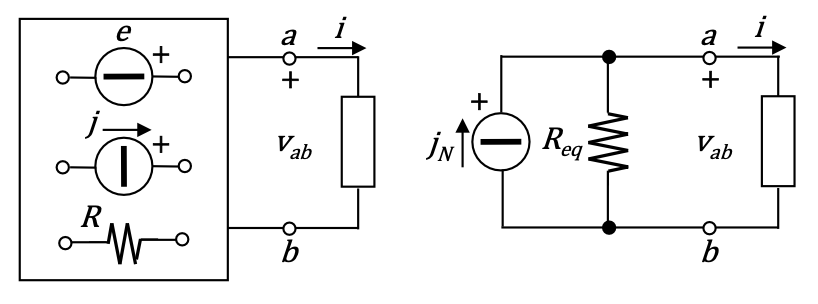
\includegraphics[scale=0.45]{immagini/Nor}
		\end{center}
		\item Equivalenza Thevenin-Norton : 
		$$E_T=R_{eq}*I_N$$
	 \end{itemize}
\end{teo*}
\begin{teo*}{Principio di Sovrapposizione}
	In un circuito resistivo lineare , qualunque tensione o corrente è la somma degli effetti dei singoli generatori indipendenti , quando agiscono uno alla volta 
	
\end{teo*}
Per analizzare un circuito con il principio di sovrapposizione bisogna : 
\begin{enumerate}
\item Inserire un generatore alla volta , con gli altri spenti , e ricavare la grandezza desiderata 
	\begin{itemize}
		\item Per spegnere un generatore di tensione , sostituirlo con un corto circuito  
		\item Per spegnere un generatore di corrente , sostituirlo con un circuito aperto 
	\end{itemize}
	\item Somma algebricamente i risultati ottenuti 
\end{enumerate}
\subsection{Misure in regimi DC}
	\begin{itemize}
	\item Voltmetro : \\
	\begin{center}
		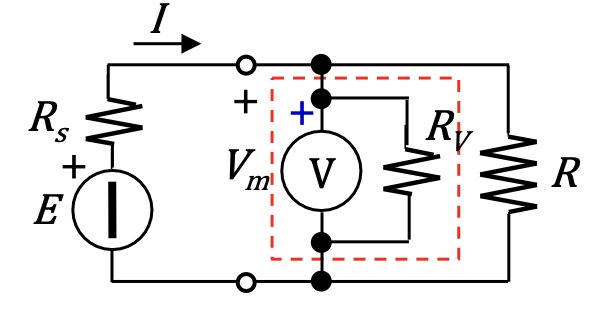
\includegraphics[scale=0.40]{immagini/volt}
	\end{center}
		\begin{align*}
		& \text{senza voltmetro} \ \ V=E\frac{R}{R+R_s}\\
		& \text{Con voltmetro ( tensione misurata )} \ \ V_m=E\frac{R || R_v}{R||R_v+R_s}\\
		& \text{errore di consumo} \ \ \epsilon_V=\frac{V_m-V}{V}=-\frac{R_s || R}{R_V+R||R_s}\approx -\frac{R_s||R}{RV}
	\end{align*}
	\item Amperometro :\\
	\begin{center}
		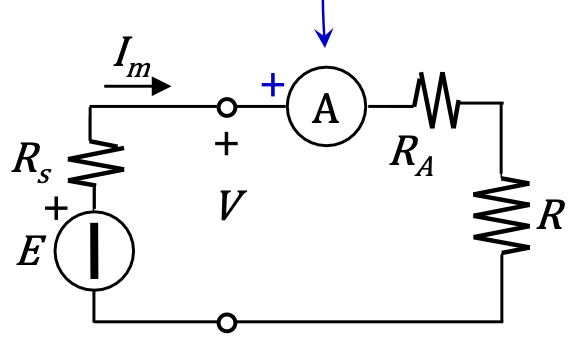
\includegraphics[scale=0.45]{immagini/amp}
	\end{center}
	\begin{align*}
		& \text{senza amperometro} \ \ I=\frac{E}{R+R_s}\\
		& \text{Con amperometro ( corrente misurata )} \ \ I_m=\frac{E}{R+R_s+R_a}\\
		& \text{errore di consumo} \ \ \epsilon_A=\frac{I_m-I}{I}=-\frac{R_a}{R_a+R+R_s}\approx -\frac{R_a}{R+R_s}
	\end{align*}
	\item Wattmetro : \\
	Nel circuiti a regime Dc possiamo calcolare la potenza in due modi completamente equivalenti : \\ utilizzando un Wattmetro o utilizzando la combinazione di un voltmetro e di un amperometro 
	\begin{center}
		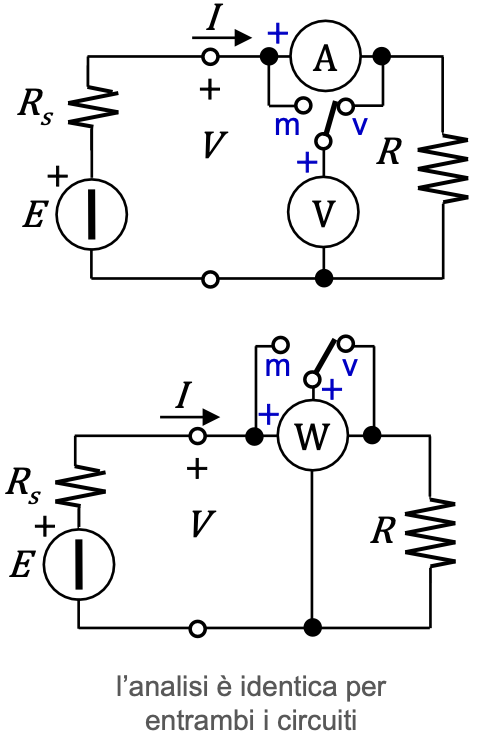
\includegraphics[scale=0.35]{immagini/wat}
	\end{center}
	Possiamo decidere in entrambi casi se collegare la parte voltmetrica o a valle o a monte ( prima o dopo l'amperometro).
	\begin{itemize}
		\item Se colleghiamo a monte è la misura della tensione che è affetta dal consumo dell'amperometro 
		$$V_m=R_AI+V \ \ \ \Delta V = R_a I \ \ \ \delta_{VA}=\frac{\Delta V}{V}=\frac{R_A}{R}$$
		\item Se colleghiamo il voltmetro a valle è la misura della corrente che è affetta da consumo del voltmetro 
		$$I_m=\frac{V}{R||R_V} \ \ \ \Delta I = \frac{V}{R_V} \ \ \ \delta_{AV}=\frac{\Delta I}{I}=\frac{R}{R_v}$$
	\end{itemize}
	\end{itemize}

\begin{teo*}{Adattamento di carico in un generatore di tensione Reale }
	Un generatore di tensione reale può essere rappresentato come generatore ideale in serie con una resistenza $R_s$  
\begin{center}
	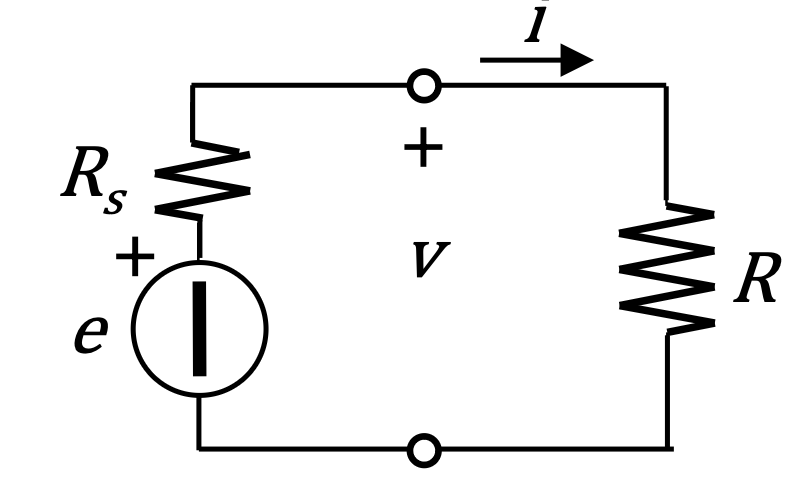
\includegraphics[scale=0.25]{immagini/real}
\end{center}
Ora sappiamo che la potenza generatore è pari a $P_g=ei=\frac{e^2}{R+R_s}$ , invece la potenza erogata al carica è $P_e=vi=RI^2=R\frac{e^2}{(R+R_s)^2}$.\\ Ora vogliamo trovare il valore di $R_s$ che massimizza la potenza trasferita al carico. Per massimizzarla imponiamo che la derivata di $P_e$ rispetto alla resistenza R sia zero e otteniamo la seguente condizione $R=R_s$\\
Tutte via nelle applicazione reali metà della potenza generata viene dissipata dalla resistenza $R_s$ , quindi spesso si preferisce un carico $R>>R_s$
\end{teo*}
\subsection{Reti del Primo ordine }
Una rete del primo ordine contiene solo un elemento reattivo (C o L) equivalente.\\
Una situazione di regime ( t < 0) è seguita da un transitorio (t=0) che termina con una nuova situazione a regime ( $ t \rightarrow \infty$)\\
Per determinare v(t) e i(t) durante il transitorio sfruttiamo la continuità della 
\begin{itemize}
\item \textbf{tensione} : sulle capacità
\item \textbf{corrente} : attraverso l'induttanza 
\end{itemize}
\subsubsection{Risposta naturale}
La risposta naturale di una rete del primo ordine rappresenta il comportamento del circuito in assenza di forzanti esterne , dipende unicamente dalle condizioni iniziali.\\
L'analisi del transitorio richiede la risoluzione di un'equazione differenziale lineare omogenea del primo ordine a coefficienti costanti  $\frac{ d x(t)}{dl t}+a x(t)=0$ che come soluzione $$x(t)=Ke^{\frac{t}{\tau}}$$ dove K è determinata dalla condizione iniziale (K=x(0))  invece $\tau=\frac{1}{a}$ è detta costante di tempo 
\paragraph{Rete RC}
\begin{center}
	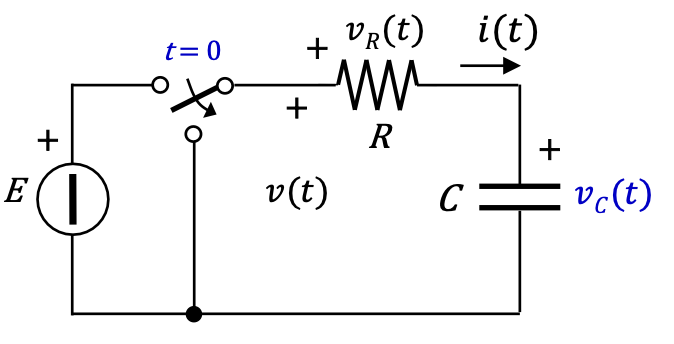
\includegraphics[scale=0.40]{immagini/rc1}
\end{center}
per $t <0$ la corrente $I(t)=0$ invece la tensione ai capi del condensatore è pari a $v_c(t)=E$\\
Ora sappiamo che per la continuità $v_c(0-)=v_c(0+)=E$ quindi sappiamo anche che $K=v_c(0)=E$\\
Invece per $t >0$ il condensatore di scarica comportandosi come un generatore quindi $v(t)=v_R+v_c=Ri+v_c=RC \dot{v_c}(t)+v_c=0$
$$\dot{v_c}(t)+\frac{1}{RC}v_c=0$$
ora abbiamo scoperto anche la costante di tempo che è $\tau=RC$ quindi possiamo scrivere la soluzione dell'equazione differenziale 
$$v_c(t)=Ke^{-\frac{t}{\tau}}=Ee^{-\frac{t}{RC}}$$
Ora che abbiamo scoperto possiamo ricavarci anche l'espressione della corrente 
sappiamo che $t<0 \ \ i(t)=0$ invece per $$t > 0 \ \ i(t)=C \dot{v}(t)=\cancel{C}E(-\frac{1}{R\cancel{C}})e^{-\frac{t}{RC}}=-\frac{E}{R}e^{-\frac{t}{RC}}$$
Ora possiamo grafare le due soluzioni : 
\begin{center}
	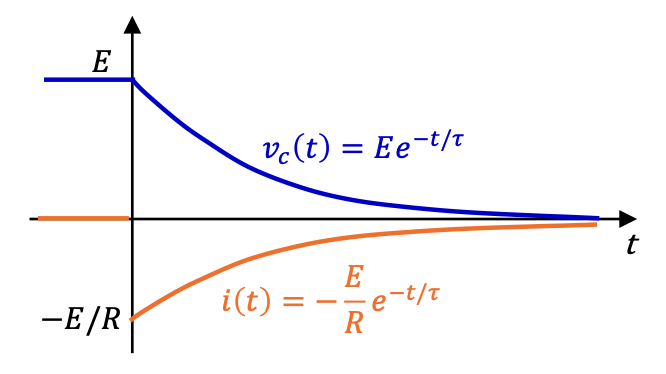
\includegraphics[scale=0.45]{immagini/g}
\end{center}
Vediamo che unicamente $v_c$ è continua , invece i presenta un salto durante il transitorio 


\paragraph{Rete RL}
\begin{center}
	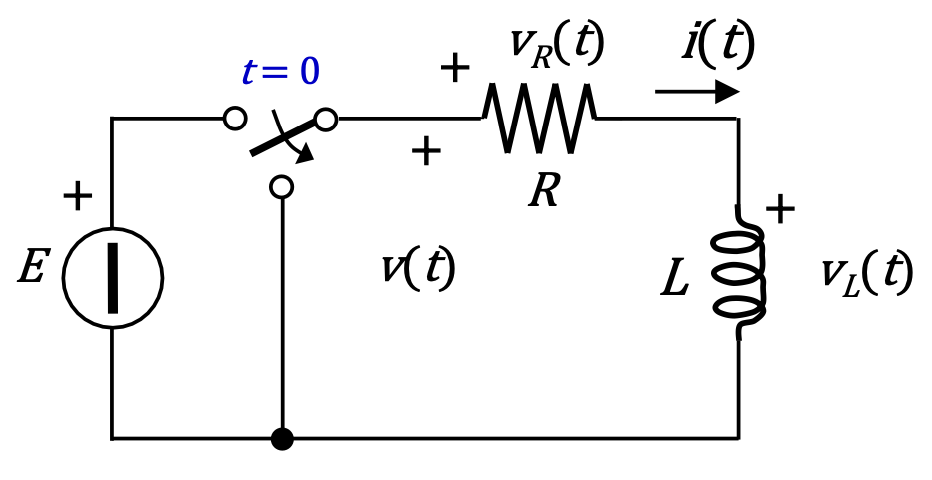
\includegraphics[scale=0.35]{immagini/rl}
\end{center}
Per $t<0 \ \ \ v_L(t)=0 \ \ i(t)=\frac{E}{R}$  \\
Inoltre sappiamo che per la continuità $i(0-)=i(0+)=\frac{E}{R}=K$ \\
Per $t>0$ l'induttanza inizia a comportarsi come un generatore di corrente quindi $v(t)=v_r+v_L=L\dot{I}(t)+I(t)R=\dot{I}(t)+\frac{R}{L}I(t)=0$ quindi ora abbiamo l'equazione differenziale $$\frac{dI}{dt}+\frac{R}{L}I(t) \ \text{la cui soluzione è :}\ I(t)=\frac{E}{R}e^{-\frac{t}{\frac{L}{R}}}$$ dove $\tau=\frac{L}{R}$ è la costante di tempo. \\
Ora che sappiamo la corrente $i(t)$ possiamo anche ricavare la tensione ai capi dell'induttore 
$$v_L(t)=L\frac{dI}{dt}=L\frac{E}{R} (-\frac{R}{L})e^{-\frac{t}{\frac{L}{R}}}=-Ee^{-\frac{t}{\frac{L}{R}}}$$
Ora possiamo grafare entrambe le curve 
\begin{center}
	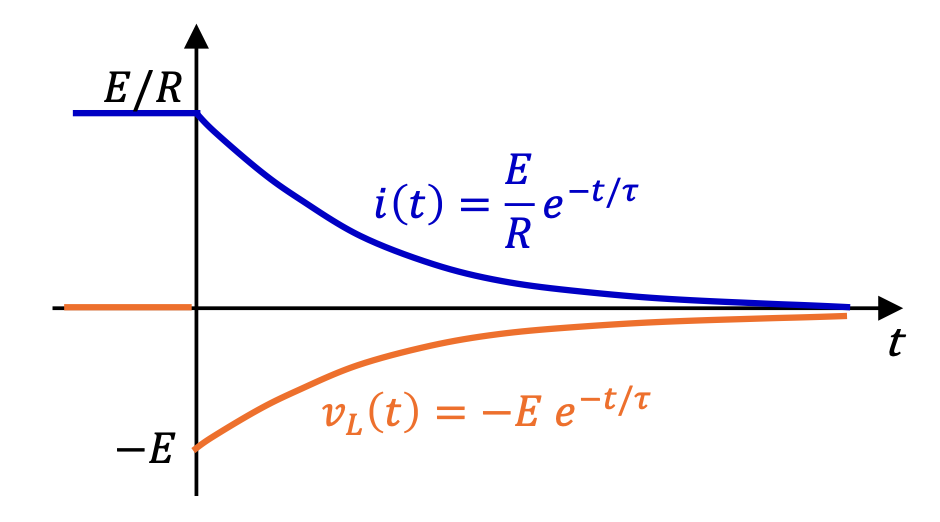
\includegraphics[scale=0.45]{immagini/gl}
\end{center}
\subsubsection{Risposta forzata}
In questo caso l'analisi del transitorio richiede la risoluzione di un'equazione differenziale lineare non omegenea del primo ordine a coefficienti costanti $$\frac{dx(t)}{t}+ax(t)=f(t)$$
Se la sollecitazione è a gradino allora la funzione $f(t)$ è costante. 
La soluzione allora è $x(t)=Ke^{-\frac{t}{\tau}}+X$
\paragraph{Reti RC}
\begin{center}
	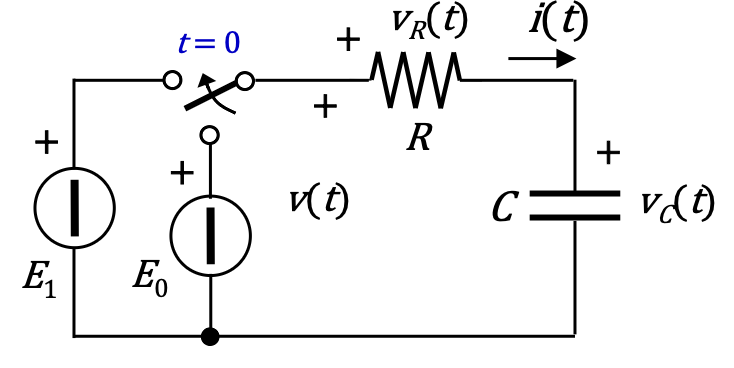
\includegraphics[scale=0.35]{immagini/rcf}
\end{center}
Per $t<0 \ \ i(t)=0 \ \ v(t)=v_r+v_c=v_c=E$\\
Ora sappiamo che per continuità $v_c(0-) =v_c(0+)=E$ \\
Per $t>0 \ \ \ v(t)=v_R+v_c=Ri+v_c=RC\dot{v_c}(t)+v_c(t)=E_1$
$$\dot{v_c}(t)+\frac{1}{RC}v_c(t)=\frac{E_1}{RC}$$
La soluzione è quindi $$v_c(t)=Ke^{\frac{-t}{\tau}}+v_c(\infty)=(E_0-E_1)e^{\frac{-t}{RC}}+E_1$$
ora che abbiamo scoperto la $v_c(t)$ possiamo ricavarci la $i(t)$
$$i(t)=C \dot{v_c}(t)=C (E_0-E_1)(-\frac{1}{RC})e^{\frac{-t}{RC}}=\frac{E_1-E_0}{R}e^{\frac{-t}{RC}}$$
Ora possiamo grafare le due soluzioni 
\begin{center}
	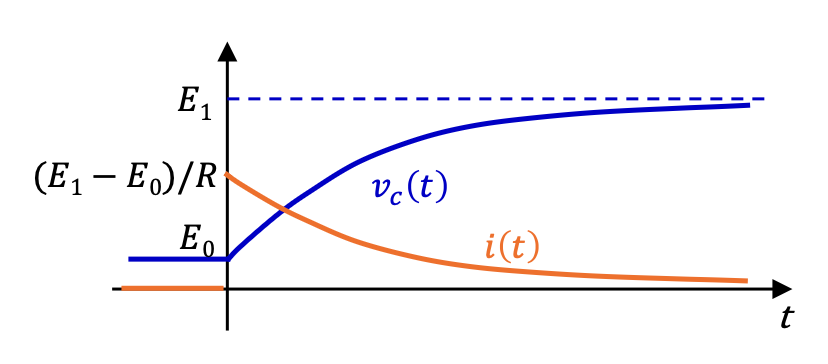
\includegraphics[scale=0.45]{immagini/gcf}
\end{center}
\paragraph{Reti RL}
\begin{center}
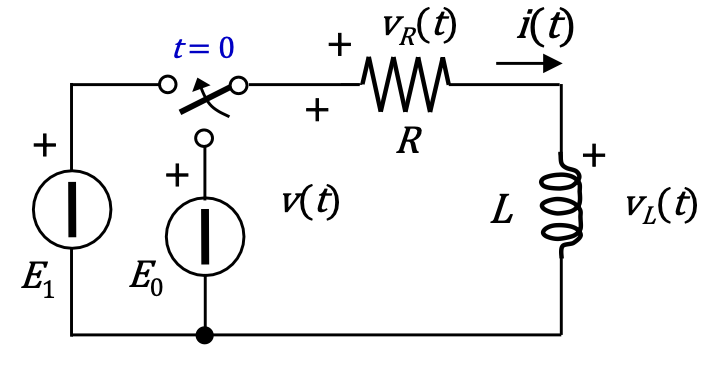
\includegraphics[scale=0.35]{immagini/rlf}
\end{center}
Per $t<0 \ \ v_L(t)=0 \ \ i(t) = \frac{E_0}{R}$\\
Ora sappiamo che per continuità $i(0+)=i(0-)=\frac{E}{R}$\\
Per $t>0 \ \ \ v(t)=v_R+v_L=RI(t)+L\frac{di}{dt}=E_1$
$$\frac{di}{dt}+\frac{R}{l}i(t)=\frac{E_1}{L}$$
La soluzione è quindi 
$$i(t)=\frac{E_0-E_1}{R}e^{-\frac{r}{\frac{L}{R}}}+\frac{E_1}{R}$$
Ora che sappiamo i(t) possiamo ricavare $v_L(t)$
$$v_L(t)=L\frac{di}{dt}=(E_1-E_0)e^{-\frac{r}{\frac{L}{R}}}$$\\
Ora possiamo grafare la soluzione
\begin{center}
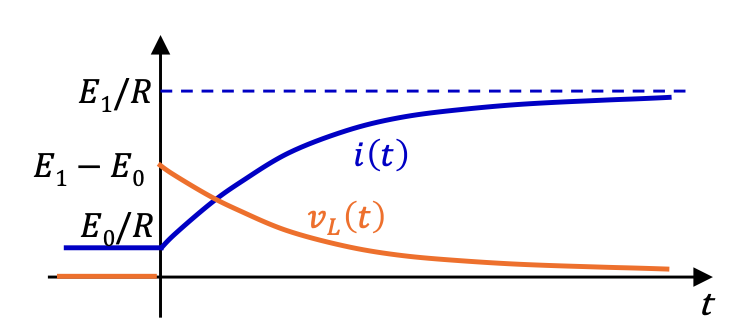
\includegraphics[scale=0.45]{immagini/glf}
\end{center}
\subsubsection{Risposta rettangolare}
Una sollecitazione a gradino si verifica quando si ha una doppia commutazione: da a in b per $t=0$ e da b in a per $t = t_1$
\paragraph{Rete RC}
\begin{center}
	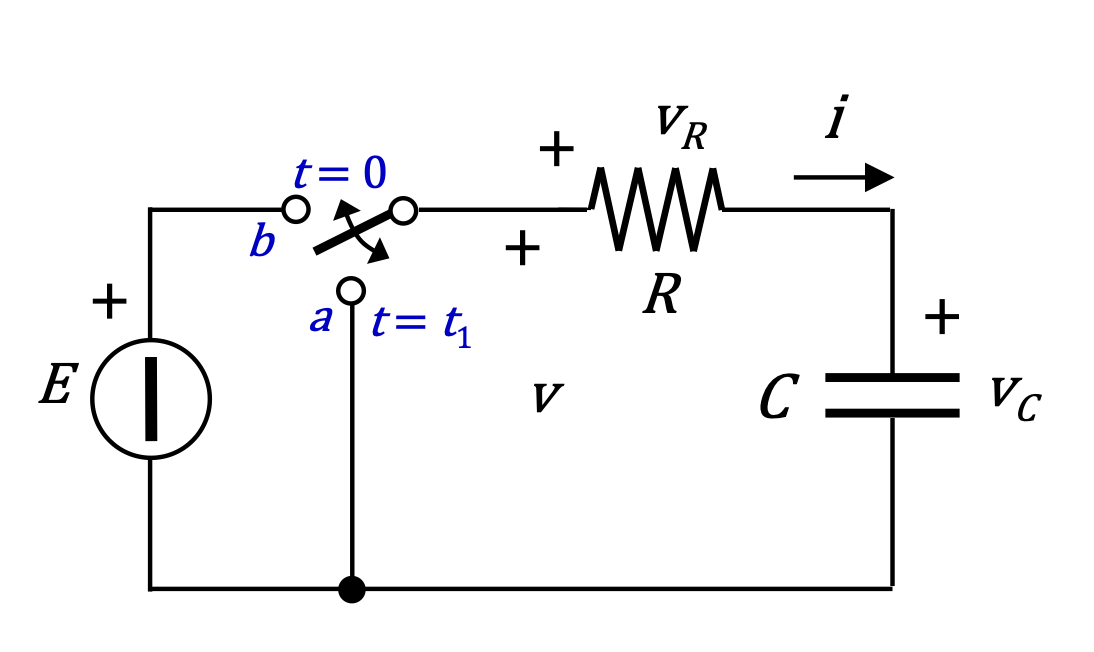
\includegraphics[scale=0.25]{immagini/sollecitazione rettangolare.png}
\end{center}
Per $t<0 \ \ v_c(t) = 0$\\
Per $0<t<t_1 \ \ v_c(t) = E(1-e^{-\frac{t}{\tau}})$ transitorio di carica\\
Per $t=t_1 \ \ v_c(t_1) = E(1-e^{-\frac{t_1}{\tau}})$\\
Per $t>t_1 \ \ v_c(t) = v_c(t_1)e^{-\frac{t-t_1}{\tau}}$ transitorio di scarica\\

Grafando la sollecitazione è:
\begin{center}
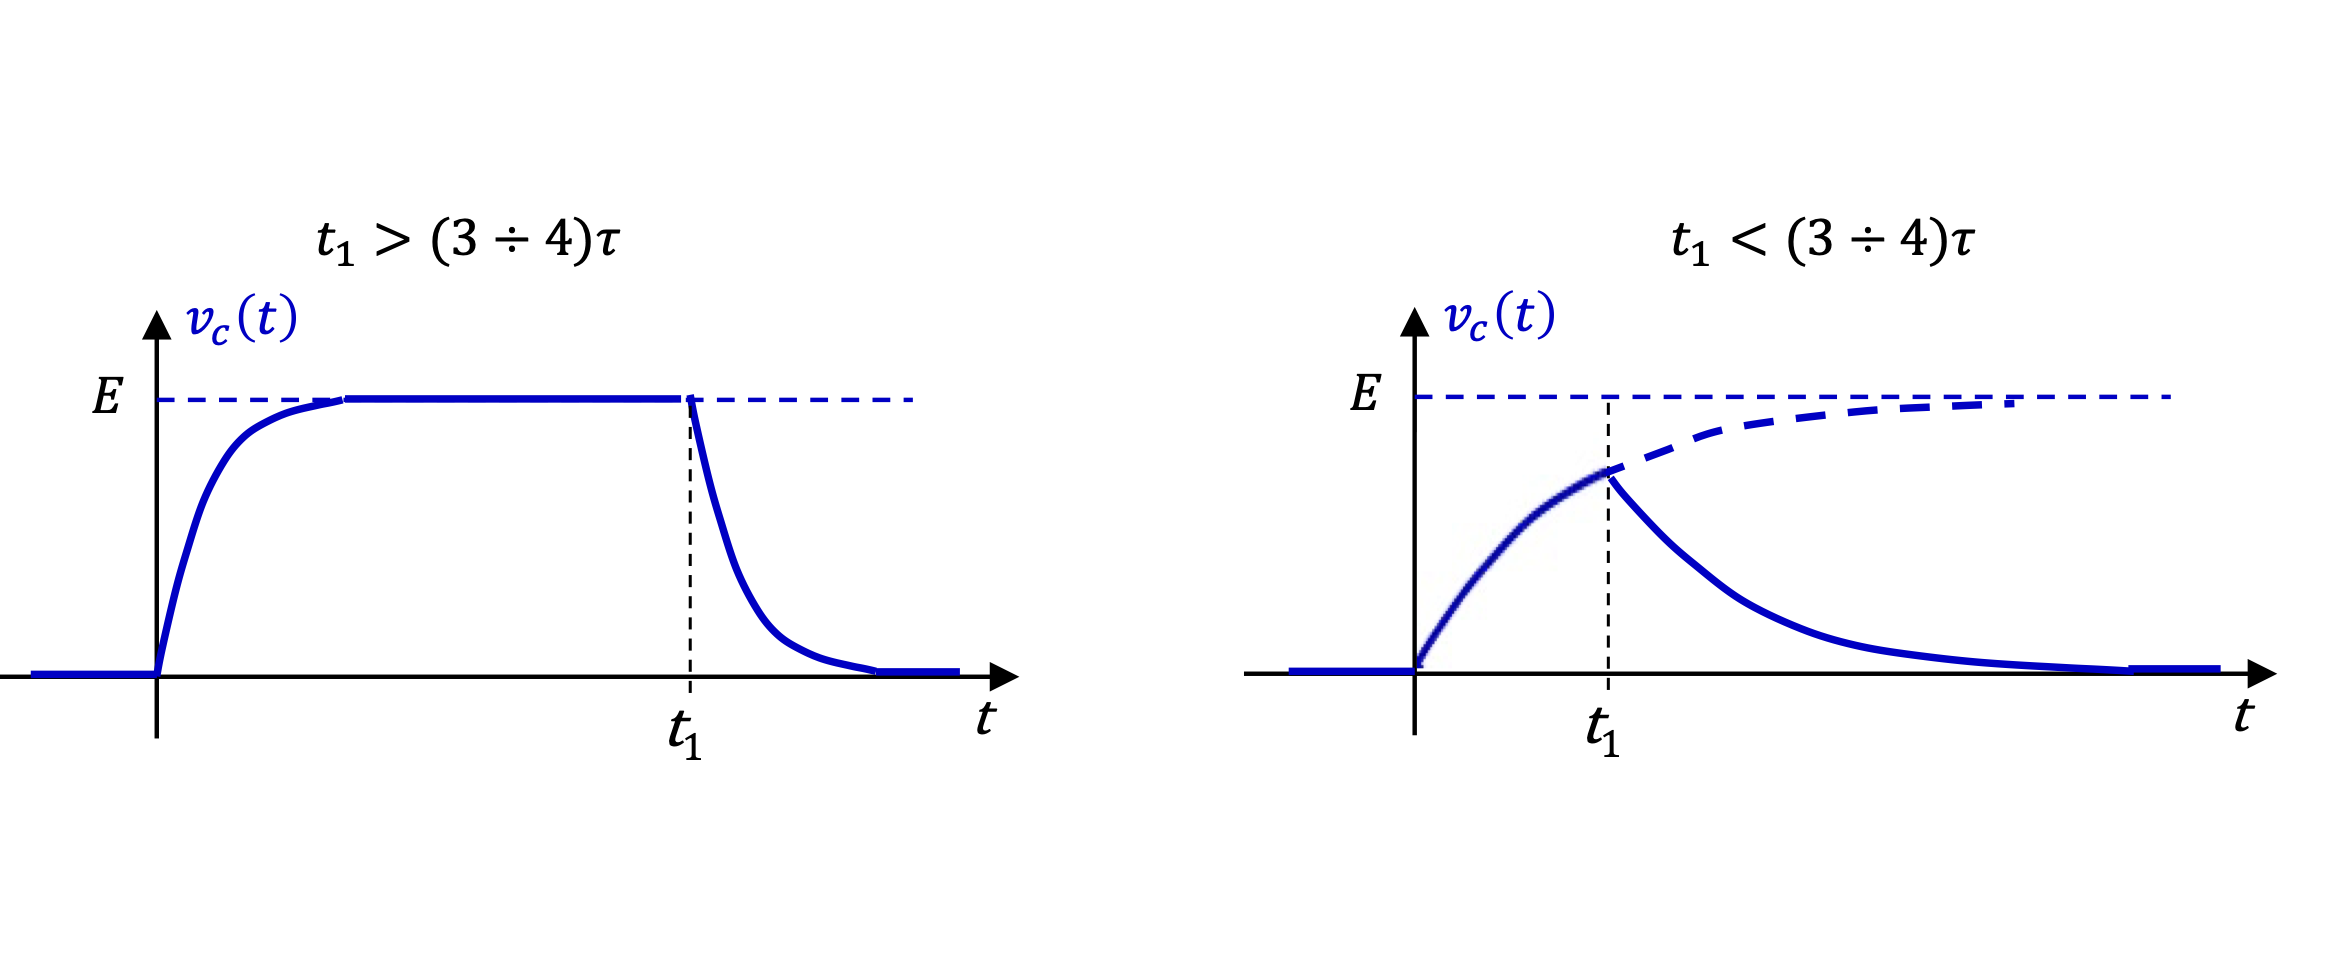
\includegraphics[scale=0.35]{immagini/grafica soll rett.png}
\end{center}
\subsection{Reti del secondo Ordine }
Le reti del secondo ordine sono reti che contengono 2 elementi reattivi diversi tra loro.\\
L'analisi del transitorio richiede la risoluzione di un'equazione differenziale lineare del secondo ordine a coefficienti costanti 
$$\frac{d^2 x(t)}{dt^2}+b\frac{d x(t)}{dt}+c x(t)=\frac{d^2 x(t)}{dt^2}+2\alpha\frac{dx(t)}{dt}+\omega^2_0 x(t)=f(t)
$$
Per le sollecitazioni a gradino abbiamo che f(t)=F cioè è costante\\
\begin{teo*}{equazione caratteristica dell'eq differenziale}
$$s^2+2\alpha s+\omega^2_0 \ \ \ \text{con} \ \ \begin{cases}
2\alpha=\frac{R}{2L}\\
w_0^2=\frac{1}{LC}
\end{cases}$$
Le cui soluzioni sono : 
$$s=-\alpha\pm \sqrt{\alpha^2-\omega^2_0}$$
\end{teo*}
Vista l'equazione caratteristica della nostra equazione differenziale possiamo avere tre diversi casi 
\begin{itemize}
\item Rete \textbf{sovrasmorzata}  ($\Delta >0$):
\tcboxmath{x(t)=K_1e^{\frac{-t}{\tau_1}}+K_2e^{\frac{-t}{\tau_2}}} \\con $\tau_1=-\frac{1}{s1} \ \ \ \tau_2=-\frac{1}{s_2}$
\item Rete a \textbf{smorzamento critico} ($\Delta = 0$):
\tcboxmath{x(t)=K_1e^{\frac{-t}{\tau}}+K_2e^{\frac{-t}{\tau}}} con $\tau=\frac{1}{\alpha}$
\item Rete \textbf{sottosmorzata} ($\Delta < 0$):
\tcboxmath{x_n(t)=K_1e^{\frac{-t}{\tau}}cos(w_nt)+K_2e^{\frac{-t}{\tau}}sin(w_nt)} con $\tau=\frac{1}{\alpha}$  e $\omega_n=\sqrt{-\Delta}$
\end{itemize}
\paragraph{RLC in serie}
\begin{center}
	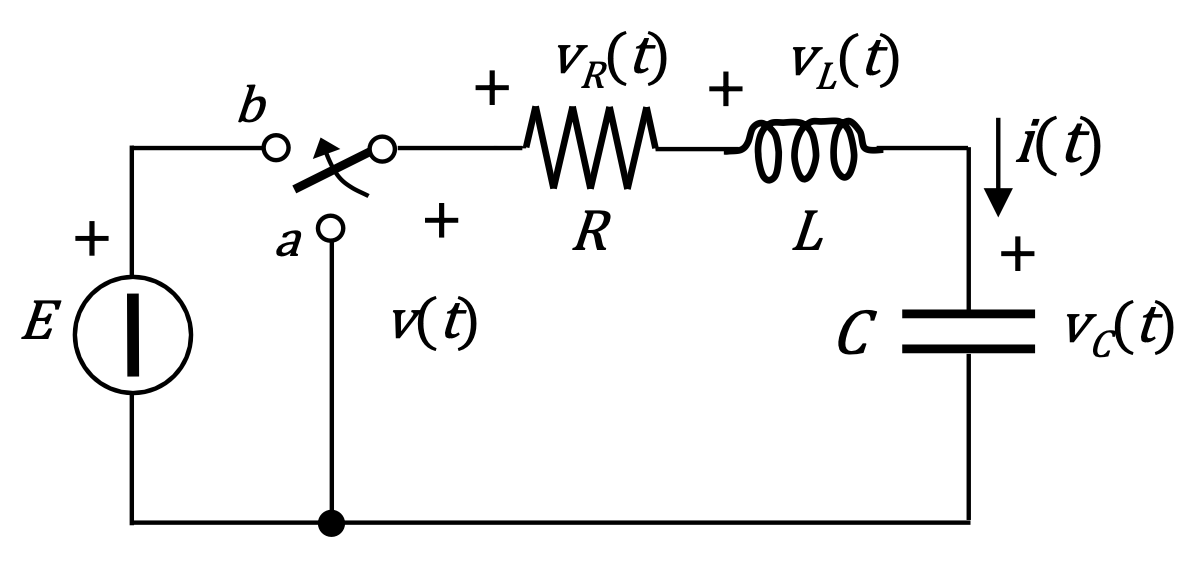
\includegraphics[scale=0.40]{immagini/rlc}
\end{center}
Per $t < 0 \ \ \ i(t)=0 \ \ \ v_c(t)=0$  inoltre $i(t) \  e  \ v_c(t)$ variano entrambe con continuità.\\
Per $t > 0 : v(t)=v_R+v_L+v_c=RC\frac{dv_(t)}{dt}+LC\frac{d^2v_c(t)}{dt^2}+v_c=E $
$$\frac{d^2v_(t)}{dt^2}+\frac{R}{L}\frac{dv_c(t)}{dt}+\frac{1}{LC}v_c=\frac{E}{LC}$$
quindi ora sappiamo che $\alpha=\frac{R}{2L} \ e \ \omega^2_0=\frac{1}{LC}$ quindi possiamo scrivere l'equazione caratteristica 
$$s_{1,2}=-\alpha \pm \sqrt{\Delta}=-\frac{R}{2L}\pm \sqrt{\left( \frac{R}{2L}\right) ^2-\frac{1}{L}}$$
\begin{enumerate}
\item$E=10V ; R=300\Omega ;L=10 mH;C=1\mu F$\\
In questo abbiamo una rete sovrasmorzata poichè $\Delta > 0 $ quindi abbiamo una soluzione del tipo 
$$v_c(t)=v_{cn}(t)+v_{cr}(t)=K_1e^{-\frac{t}{\tau_1}}+K_2e^{-\frac{t}{\tau_2}}+E$$ inoltre dalle condizioni iniziali possiamo ricavare $K_1 \ e \ K_2$ \\
	$v_c(0)=K_1+K_2+10  i(0)=C\frac{dv_c}{dt}=-\frac{K_1}{\tau_1}-\frac{K_2}{\tau_2}=0$ da cui ricaviamo che $K_1=1.7V \ K_2=-11.7 V$ \\
	Ora possiamo grafare la soluzione :
	\begin{center}
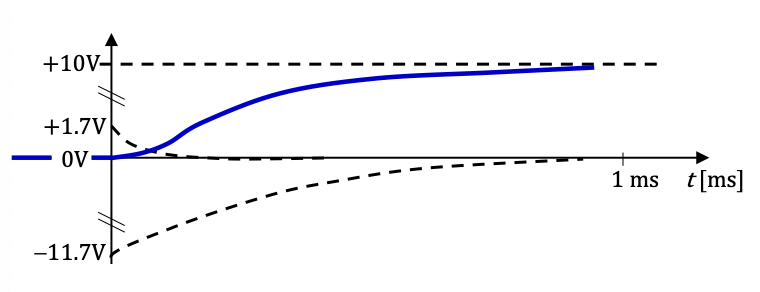
\includegraphics[scale=0.40]{immagini/sovra}
	\end{center}
\item $E=10V ; R=200\Omega ;L=10 mH;C=1\mu F$\\
In questo caso abbiamo una retta a smorzamento critico poichè $\Delta =0$
quindi abbiamo una soluzione del tipo : 
$$v_c(t)=v_{cn}(t)+v_{cr}(t)=K_1e^{\frac{-t}{\tau}}+K_2e^{\frac{-t}{\tau}} +E$$
Inoltre dalle condizioni iniziali possiamo ricavare $K_1 \ e \ K_2$ \\
$v_c(0)=K_1+10=0 \ \  i(0)=C\frac{dv_c}{dt}=-\frac{K_1}{\tau}+K_2=0$ da cui ricaviamo che $K_1=-10V \ K_2=-10^5 V$ \\
Ora possiamo grafare la soluzione :
\begin{center}
	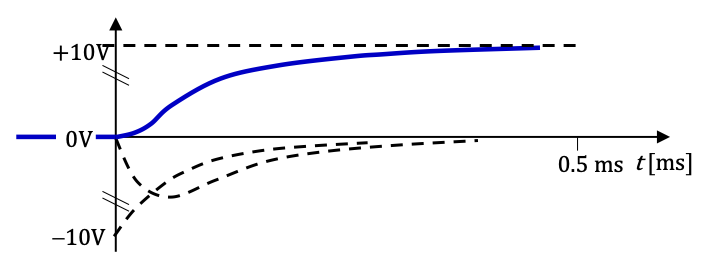
\includegraphics[scale=0.40]{immagini/critico}
\end{center}
\item $E=10V ; R=100\Omega ;L=10 mH;C=1\mu F$\\
In questo caso abbiamo una rete sottosmorzata poichè $\Delta < 0$ quindi abbiamo una soluzione del tipo 
$$v_c(t)=K_1e^{\frac{-t}{\tau}}cos(w_nt)+K_2e^{\frac{-t}{\tau}}sin(w_nt)+E$$
Inoltre dalle condizioni iniziali possiamo ricavare $K_1 \ e \ K_2$ \\
$v_c(0)=K_1+10=0 \ \  i(0)=C\frac{dv_c}{dt}=-\frac{K_1}{\tau}+\omega_nK_2=0$ da cui ricaviamo che $K_1=-10V \ K_2=-5.8V$ \\
Ora possiamo grafare la soluzione :
\begin{center}
	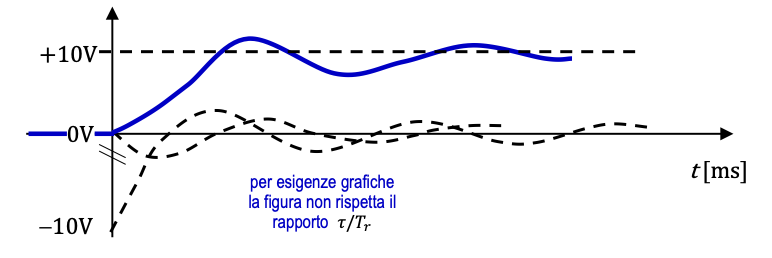
\includegraphics[scale=0.50]{immagini/sottosmorzato}
\end{center}
\begin{figure}[h]
	\centering
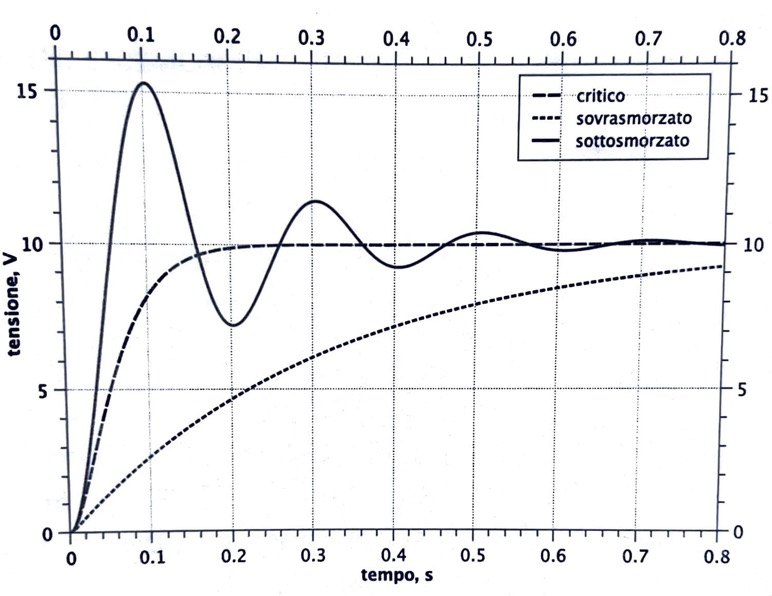
\includegraphics[scale=0.30]{immagini/totale}
\caption{confronto fra l'andamento della tensione sul condensatore nei tre casi descritti}
\end{figure}
\end{enumerate}
\newpage
\section{Circuiti in AC}
\subsection{Relazione caratteristiche degli elementi passivi }
\begin{center}
\begin{tabular}{|c|c|c|}
	\hline
	\rule[-1ex]{0pt}{2.5ex}  &Dominio del Tempo  & Dominio della frequenza   \\
	\hline
	\rule[-1ex]{0pt}{2.5ex}  Resistore &$v(t)=Ri(t)$  & $V=RI$  \\
	\hline
	\rule[-1ex]{0pt}{2.5ex} Induttore  &$v(t)=L\frac{di(t)}{dt}$  &$V=j\omega I$  \\
	\hline
	\rule[-1ex]{0pt}{2.5ex}  Capacità &$i(t)=\frac{dv(t)}{dt}$  &$V=-\frac{j}{\omega C} I$ \\
	\hline
\end{tabular}
\end{center}
Inoltre possiamo anche vedere che per l'induttore \textbf{la corrente è in ritardo rispetto alla tensione} invece per il condensatore \textbf{la corrente è in anticipo rispetto alla tensione }.Invece per la resistenza \textbf{corrente e tensione sono in fase} \\
Quindi anche l'induttore e il condensatore in regime sinusoidale seguono una legge di Ohm simbolica che in generale può essere scritta come 
$$V=ZI$$ essendo 
\begin{center}
	
\begin{tabular}{|c|c|}
	\hline
	$Z=R$ & per il resistore \\
	\hline
	$Z=j\omega L$ &per l'induttore   \\
	\hline
	$Z=\frac{1}{j \omega C}$ &  per il condensatore \\
	\hline
\end{tabular}
\end{center}
La quantità \textbf{Z} prende il nome di impedenza dell'elemento ( si misura in Ohm)  e può essere invertita definendo così la quantità Y chiamata ammettenza.\\
Le regole di composizione di resistenze in serie o in parallelo si estendono anche ai circuiti simbolici, purchè si faccia riferimento alle impedenze o alle ammettenze. \\
Quindi : \begin{itemize}
	\item Impedenze in serie: 
	$$Z_{eq}=\sum_{k=1}^nZ_k$$
	\item Impedenze in parallelo :
	$$\frac{1}{Z_{eq}}=\sum_{k=1}^{n}\frac{1}{Z_k}$$
	\end{itemize}
\subsection{Teorema del generatore equivalente}
Il teorema di Thevenin si applica anche ai circuiti simbolici. In tal caso la tensione a vuoto è un fasore  e al posto della resistenza equivalente si ha un'impedenza equivalente.Discorso analogo si applica al  teorema di Norton , in tal caso la corrente è un fasore e al posto della resistenza equivalente si ha un'altra impedenza equivalente.
\subsection{Potenza}
\subsubsection{Potenza istantanea}
$$p(t)=v(t)i(t)=2VIcos(\omega t+\phi_v)cos(\omega t +\phi_i)=VIcos(\phi_v-\phi_i)+VIcos(2\omega+\phi_v+\phi_i)$$
Chiamiamo $\phi=\phi_v-\phi_i$ lo sfasamento tra tensione e corrente e inoltre chiamiamo $cos(\phi)$ il fattore di potenza.
\subsubsection{potenza media/attiva/reale}
Il fattore $VIcos(\phi)$ è la \textbf{potenza media/attiva/reale}  che rappresenta la potenza reale consumata dal carico per svolgere lavoro utile, come riscaldamento, illuminazione o movimento meccanico.
$$P=\left\langle p(t)\right\rangle =\frac{1}{T}\int_0^Tp(t)dt=VIcos(\phi)\ \ [W]$$
P fissata  , se anche V è fissata :
\begin{itemize}
	\item se $\phi=0$ ( carico resistivo) , P è trasferita con I (ed S) minima
	\item se $\phi\neq0$ (carico reattivo) I (ed S) aumenta e rispetto a valore strettamente necessario per trasferire una data P.
\end{itemize}
Il fattore $VIcos(2\omega+\phi_v+\phi_i)$ è la componente fluttuante che "rimbalza" tra carico e sorgente con frequenza $2\omega$.
\subsubsection{potenza apparente}
La \textbf{potenza apparente}  è $$S=VI=\sqrt{P^2+Q^2} \ \ [VA]$$\\
È la combinazione vettoriale della potenza attiva e reattiva. Rappresenta la potenza totale che il sistema deve fornire.
\subsubsection{potenza reattiva}
La \textbf{potenza reattiva } è $$Q=VIsin(\phi)\ \ [VAR]$$
Indica la potenza che oscilla tra la sorgente e i componenti reattivi del circuito, come induttori e condensatori. Non produce lavoro utile ma è necessaria per il funzionamento del circuito.\\
Q rappresenta solo l'ampiezza $p_r(t)$ è improprio parlare di potenza reattiva assorbita/erogata , ma l'espressione è usata per comodità di linguaggio.
\begin{itemize}
	\item Q > 0 per l'ìinduttore 
	\item Q < 0 per il condensatore
\end{itemize}
\subsubsection{potenza nel dominio della frequenza}
La \textbf{potenza complessa} è $$\dot{S}=\dot{V}\dot{I}^*=P+jQ\ \ [VA]$$
inoltre possiamo scrivere :
$$P=Re[\dot{S}] \ \ \ e \ \ \ Q=Im [\dot{S}]$$

\newpage
\subsection{Misure in corrente alternata}
\begin{figure}[h]
\centering
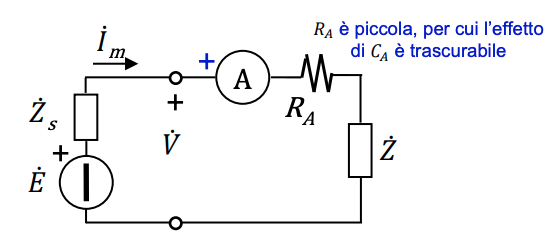
\includegraphics[scale=0.30]{immagini/ampAC}
\label{fig:1}
\hfil
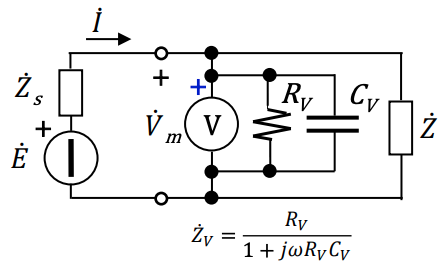
\includegraphics[scale=0.30]{immagini/voltAC}
\label{fig:2}
\end{figure}
$$\epsilon_a=\frac{\Delta_a}{|\dot{I}|}=\frac{|\dot{I}_m|-|\dot{I}|}{|\dot{I}|}\approx -\frac{R_a}{|\dot{Z}+\dot{Z}_s|} \ \ \ \ R_a <<|\dot{Z}+\dot{Z}_s|\ \ \ \ \ \ref{fig:1}$$

$$\epsilon_v=\frac{v}{\abs{\dot{V}}}=\frac{|\dot{V}_m|-|\dot{V}|}{|\dot{V}|}\approx \abs{\frac{\dot{Z}_s||\dot{Z}}{\dot{Z_v}}}\ \ \ \ \ref{fig:2}$$
\vspace{0.2cm}
\begin{figure}[h]
\centering
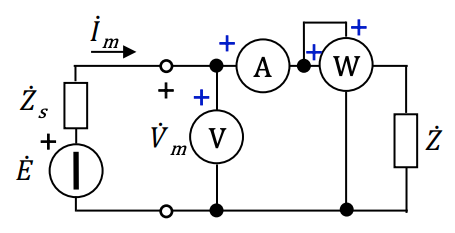
\includegraphics[scale=0.35]{immagini/wattAC}
\end{figure}

In questo caso è possibile usare solo il voltmetro e l'amperometro se essi misurano $\dot{V}_M , \dot{I}_M$ , cioè sono Phasor Measurement unit , che però per funzionare hanno bisogno dello stesso riferimento temporale che viene preso tramite GPS
\subsubsection{Multimetri digitali }
Le incertezze sono di tre tipi :
\begin{itemize}
	\item Incertezza strumentale
	\item Incertezza di interazione 
	\item Incertezza di definizione
\end{itemize}.
L'incertezza strumentale di un DMM si può calcolare come 
$$\Delta=k_1\abs{x_{mis}}+k_0R$$
dove $k_1,k_0$ sono costanti , $x_{mis}$ è il valore assoluto della misura effettuata e e infine R è portata o il range scelto (es:10V,100V)\\
Inoltre l'incertezza totale può essere vista come :
$$\Delta_{tot}=\Delta+\Delta_t=(k_1\abs{x_{mis}}+k_0R)+(k_{1T}\abs{x_{mis}}+k_{0T}R+\abs{\abs{T-T_{cal}}-5C})$$
dove T è la temperatura attuale di lavoro e $T_{cal}$ è la temperatura di calibrazione.\\
Infatti , per l'incertezza strumentale , le due principali grandezze di influenza sono la temperatura e il tempo trascorso dalla taratura 
\newpage
\subsubsection{Adattamento di carico in  AC}
\begin{wrapfloat}{figure}{I}{0pt}
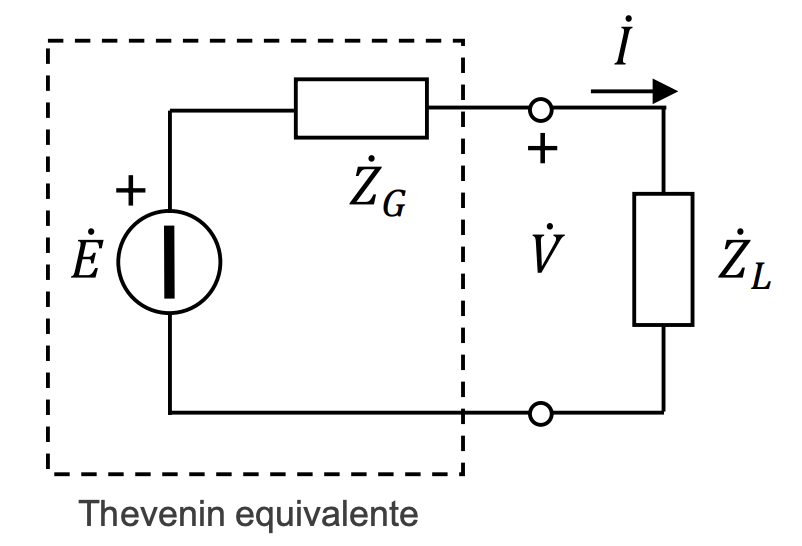
\includegraphics[scale=0.30]{immagini/AC}
\end{wrapfloat} 

$$\dot{I}=\frac{\dot{E}}{\dot{Z_G}+\dot{Z_L}} \ \ \ I=\frac{E}{\sqrt{(R_G+R_L)^2+(X_G+X_L)^2}}$$ 
$$P=R_LI^2=\frac{E^2R_L}{(R_G+R_L)^2+(X_G+X_L)^2}$$
Abbiamo che la potenza massima viene trasferita quando l'impedenza del carico è uguale al complesso coniugato dell'impedenza  della sorgente. : $Z_L=Z_G^*$.
\\Quindi sapendo che $Z_L=R_L+X_L \ e\ Z_G^*=R_G-X_G $  possiamo dire che 
$$R_L=R_G \ e \ X_L=-X_G$$
Quindi la potenza massima è $P_{max}=\frac{E^2}{4R_L} \ \ P_g=\frac{E}{2R_L} \  \  \eta=50\% $
\subsubsection{Rifasamento}
Il rifasamento è la tecnica utilizzata per ridurre la potenza reattiva assorbita dal carico e quindi migliorare il fattore di potenza $cos(\phi)$. In Europa il fattore di potenza obbiettivo è $cos(\phi')=0.95$.
\begin{itemize}
\item Caso carico induttivo:\\
La maggior parte due carichi industriali è induttiva e introduce un ritardo nella corrente rispetto alle tensione. Per rifasare il sistema si installano condensatori in parallelo rispetto al carico 
\item Caso carico capacitivo : \\
Se il sistema è capacitivo viene invece introdotto un induttore in parallelo o in serie rispetto al carico 
\end{itemize}
Data un certo $\phi \ e \ \phi'$ possiamo calcolare la capacità del condensatore utile ad avere $\phi'$.
$$C=\frac{R}{\omega Z^2}(tan(\phi)-tan(\phi'))$$
\subsection{Filtri}
\begin{definizione}
sistema lineare stazionario con memoria: sistema che è \begin{itemize}
\item lineare : soddisfa il principio di sovrapposizione 
\item stazionario : il comportamento del sistema non cambia con il tempo 
\item con memoria: l'output $y(t)$ non dipende unicamente dall'input attuale ma anche dai valori passati/futuri dell'input 
\end{itemize}
\end{definizione}
Se abbiamo in ingresso e in uscita la stessa grandezza allora abbiamo un \textbf{filtro}\\
I sistemi sono descritti da : 
\begin{itemize}
	\item nel tempo dall'integrale di convoluzione :
	$$y(t)=\int_{-\infty}^{\tau}x(\tau)h(t-\tau)d\tau$$
	dove x(t) è l'input , invece h(t) è la risposta del sistema all'impulso (che è una funziona caratteristica dell'insieme)
	\item In frequenza : grazie alla trasformata di Fourier possiamo trasformare l'integrale di convoluzione in una moltiplicazione
	\begin{center}
		\tcboxmath{\dot{Y}(\omega)=\dot{H}(\omega)\dot{X}(\omega) \ \ \ \ \dot{H}(\omega)=\frac{\dot{Y}(\omega)}{\dot{X}(\omega)}}
        \label{risposta in frequenza}
	\end{center}
    
	dove $\dot{H}(\omega)$ si chiama\textbf{ riposta in frequenza} (caratteristica del sistema )  che fornisce la dipendenza di una grandezza sinusoidale in uscita al variare della frequenza di una grandezza sinusoidale d'ingresso. Inoltre essa è una funzione complessa
\end{itemize}
\subsubsection{Risonanza}
\begin{itemize}
\item \textbf{LC in serie} 
\begin{center}
	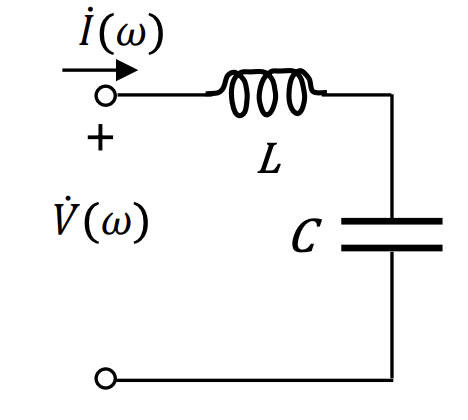
\includegraphics[scale=0.35]{immagini/LC}
\end{center}
$$Z(\omega)=j(\omega L-\frac{1}{\omega C})$$  quindi esiste un valore della frequenza tale che per cui $|Z(\omega)|=0$ e questo valore è $$\omega_0=\frac{1}{\sqrt{LC}}$$ per questo valore la reattanza induttiva compensa la reattanza capacitiva e la rete si comporta come un cortocircuito.
\begin{figure}[h]
	\centering
	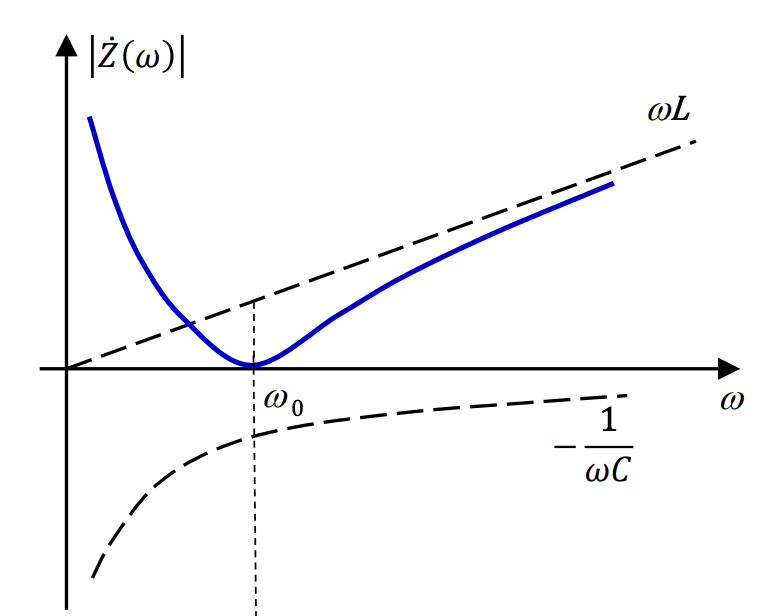
\includegraphics[scale=0.35]{immagini/1}
	\hfill
	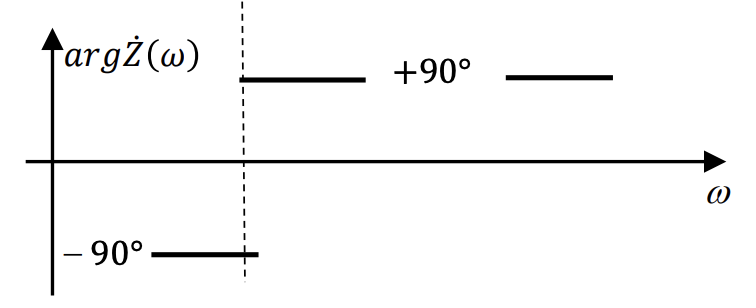
\includegraphics[scale=0.50]{immagini/2}
	\caption{Andamento del modulo dell'impedenza e del suo argomento}
	\end{figure} 
	\item \textbf{RLC in serie :}
	\begin{center}
	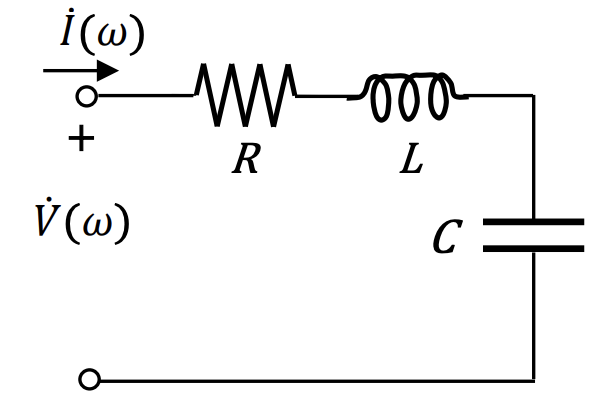
\includegraphics[scale=0.30]{immagini/RLC1}
	\end{center}
$$Z(\omega)=R+j(\omega L-\frac{1}{\omega C})$$
In questo caso la frequenza di risonanza è sempre $\omega_0=\frac{1}{\sqrt{LC}}$ ma in questo caso $|Z(\omega_0)|\neq  0 \ ma \ |Z(\omega_0)|=R \ $ \\
Inoltre possiamo scrivere l'impedenza come 
$$Z(\omega)=R\left[ 1+jQ_s\left( \frac{\omega}{\omega_0}-\frac{\omega_0}{\omega}\right) \right] $$
dove $Q_s=\frac{\omega_0L}{R}=\frac{1}{R}\sqrt{\frac{L}{C}}$ è detto fattore di qualità del circuito risonanza in serie 
\begin{figure}[h]
	\centering
	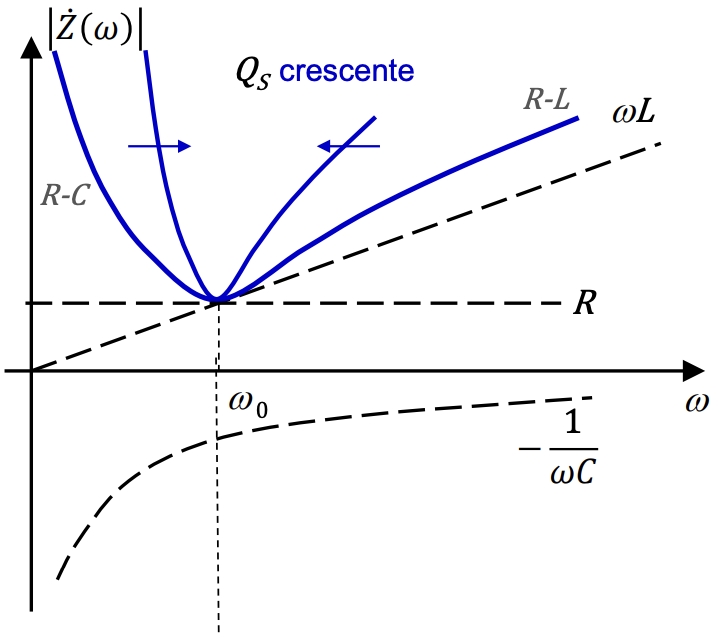
\includegraphics[scale=0.35]{immagini/3}
	\hfil
	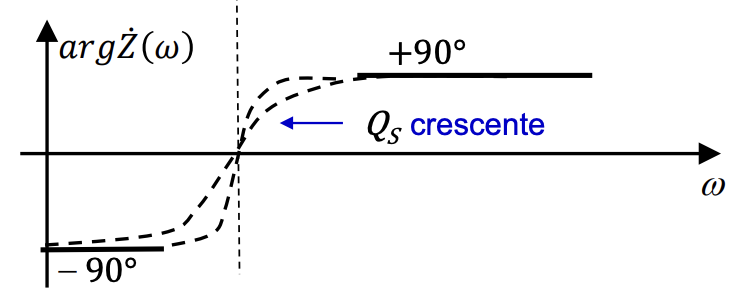
\includegraphics[scale=0.50]{immagini/4}
\end{figure}
\newpage
\item  Risonanza LC in parallelo 
Vi è un comportamento duale rispetto alla risonanza LC in serie
\begin{center}
	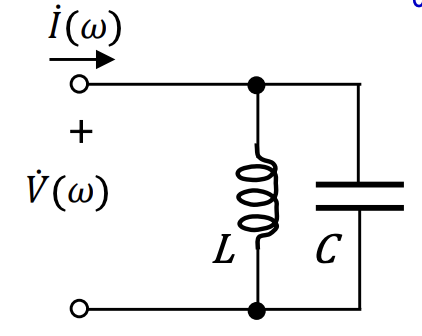
\includegraphics[scale=0.35]{immagini/LC!}
\end{center}
$$Z(\omega)=-j\frac{L/C}{\omega L -\frac{1}{\omega C}}$$
in questo caso alla frequenza di risonanza $\omega_0=\frac{1}{\sqrt{LC}}$ l'impedenza presenta un asintoto verticale infatti $|Z(\omega_0)|=+\infty$, quindi la reattanza induttiva compensa la reattanza capacitiva e il circuito si comporta come un \textbf{circuito aperto}
\begin{figure}[h]
	\centering
	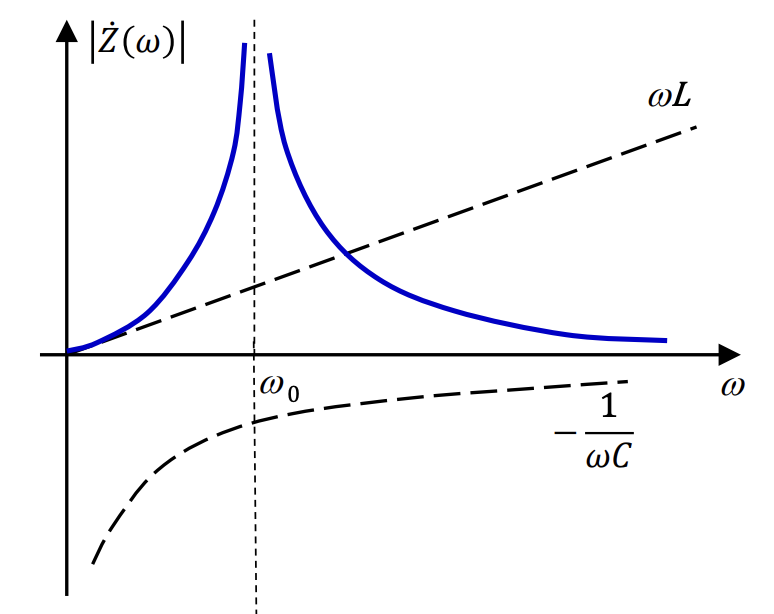
\includegraphics[scale=0.30]{immagini/5}
	\hfil
	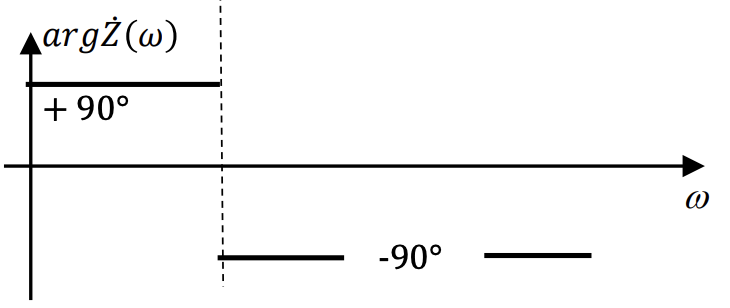
\includegraphics[scale=0.50]{immagini/6}
	\caption{Grafici del modulo e dell'argomento dell'impedenza}
\end{figure}
\item \textbf{RLC in parallelo} 
\begin{center}
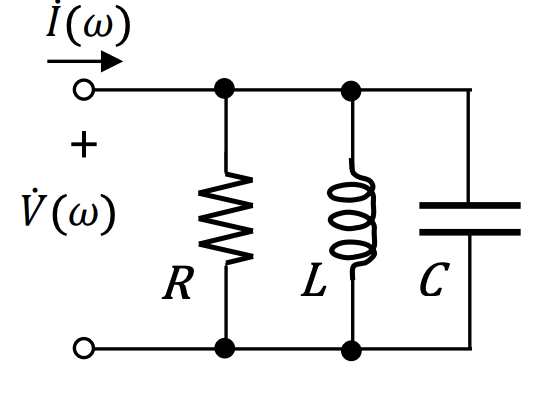
\includegraphics[scale=0.35]{immagini/RLC2}
\end{center}
$$Z(\omega)=\frac{R\frac{L}{C}}{\frac{L}{C}+jR\left(\omega L -\frac{1}{\omega C} \right) }$$
In questo caso alla frequenza di risonanza il modulo dell'impedenza non presenta un asintoto ma presenta un punto di massimo assoluto infatti $|Z(\omega_0)|=R$ .\\
Inoltre possiamo scrivere l'impedenza come 
$$Z(\omega)=\frac{R}{\left[ 1+jQ_p\left( \frac{\omega}{\omega_0}-\frac{\omega_0}{\omega}\right) \right]}$$
dove $Q_p=\frac{R}{\omega_0 L}=r\sqrt{\frac{C}{L}}$ è il fattore di qualità del circuito risonanza in parallelo 
\begin{figure}[h]
	\centering
	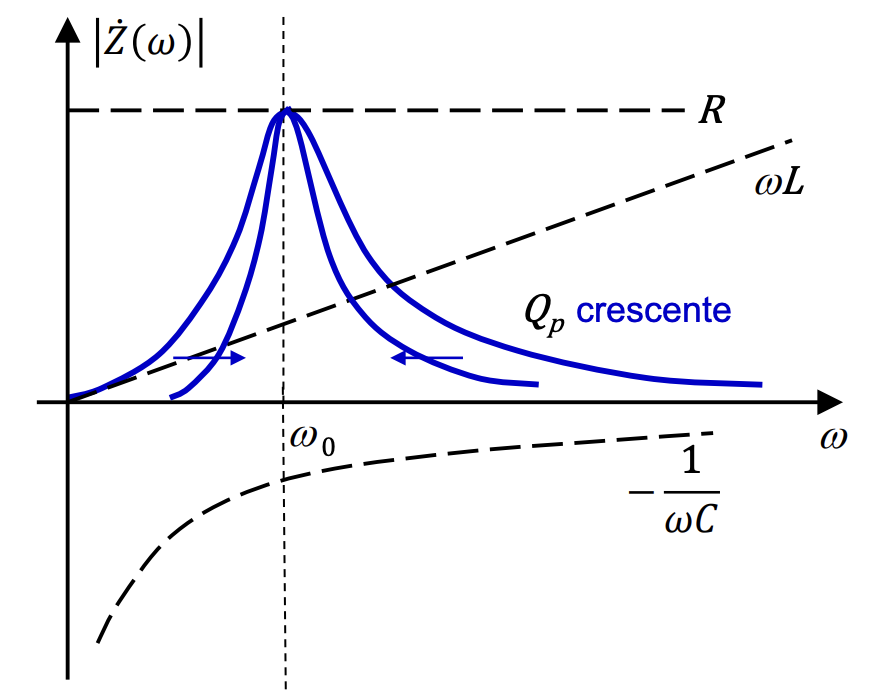
\includegraphics[scale=0.25]{immagini/7}
	\hfil
	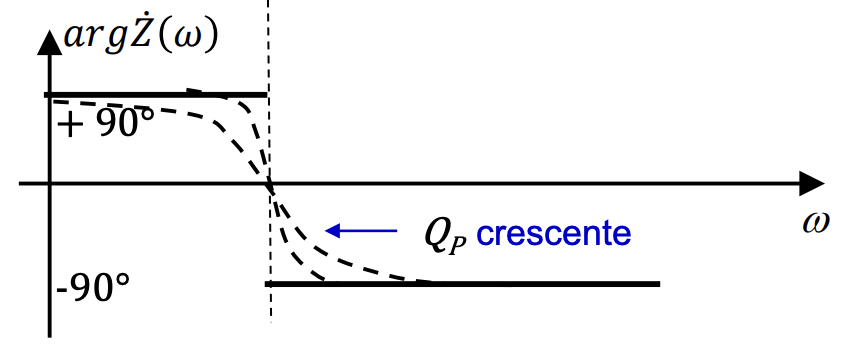
\includegraphics[scale=0.25]{immagini/8}
\end{figure}
\subsubsection{Filtri}
\textbf{N.B:} tutte le grandezze vanno intese come FASORI ( ricordatelo ti prego) stai zitto
	\begin{center}
	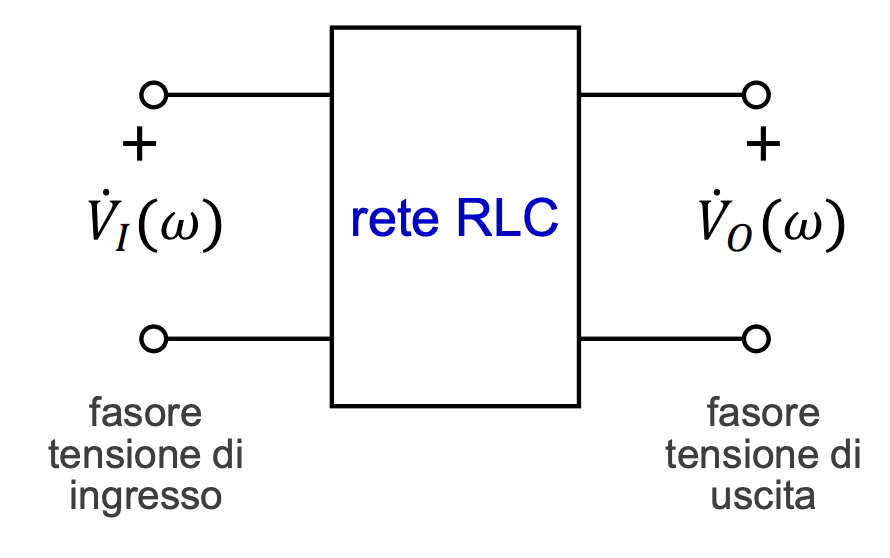
\includegraphics[scale=0.35]{immagini/bipolo}
\end{center}
Sappiamo che la risposta in frequenza si può definire come 
$$H(\omega)=\frac{V_0(\omega)}{V_I(\omega)}$$\ref{risposta in frequenza}
\begin{itemize}
\item \textbf{Filtro Passa-basso RC:} \\

\begin{center}
	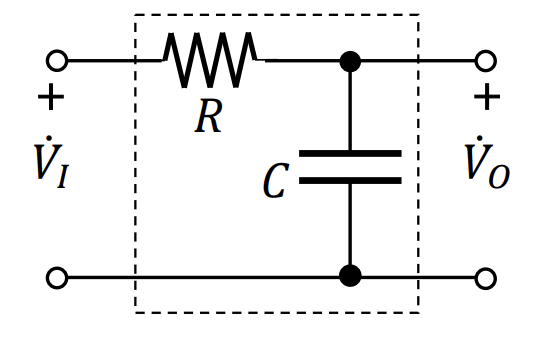
\includegraphics[scale=0.50]{immagini/pb}
\end{center}
Possiamo scrivere quindi la frequenza di risposta come 
$$H(\omega)=\frac{V_0(\omega)}{V_I(\omega)}=\frac{Z_2}{Z_1+Z_2}=\frac{\frac{1}{j\omega C}}{R+\frac{1}{j\omega C}}=\frac{1}{1+Rj\omega C}{=\frac{1}{1+j\frac{\omega}{\omega_0}}} \ \ \ \omega_0=\frac{1}{RC}$$
Possiamo inoltre definire la frequenza di taglio come 
$$f_0=\frac{\omega_0}{2\pi}$$
\begin{figure}[h]
	\centering 
	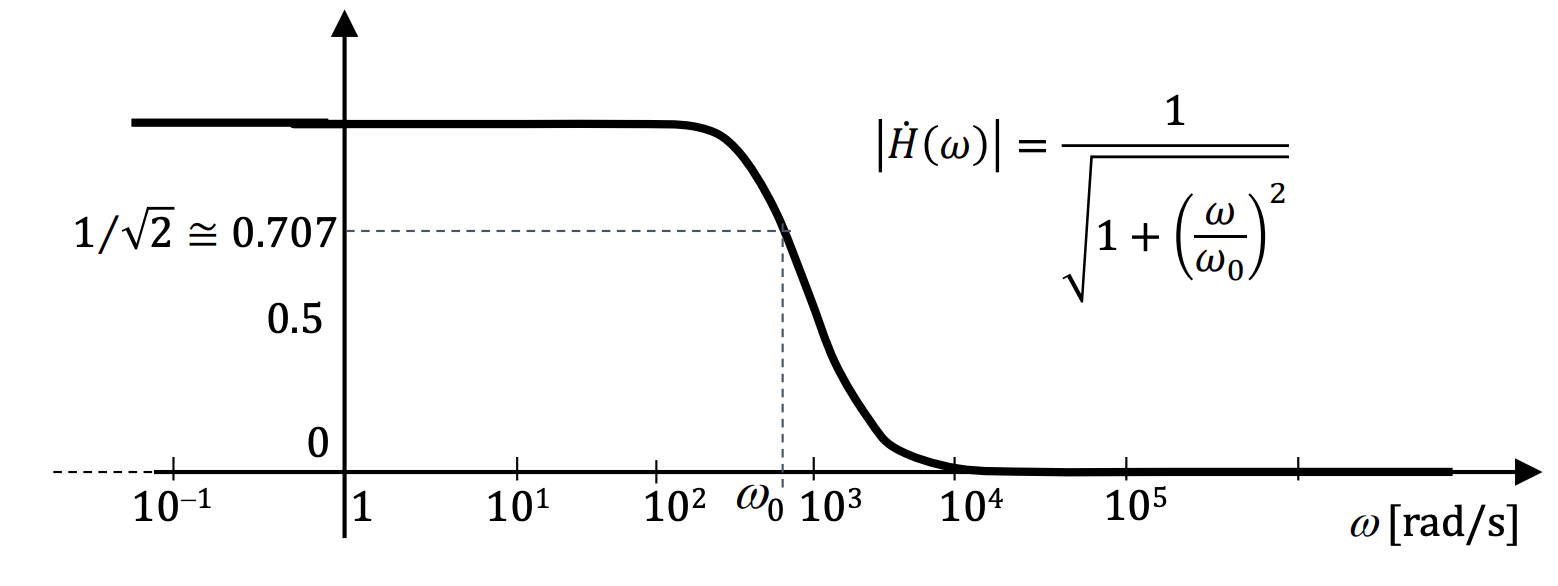
\includegraphics[scale=0.25]{immagini/pbg}
	\hfil 
	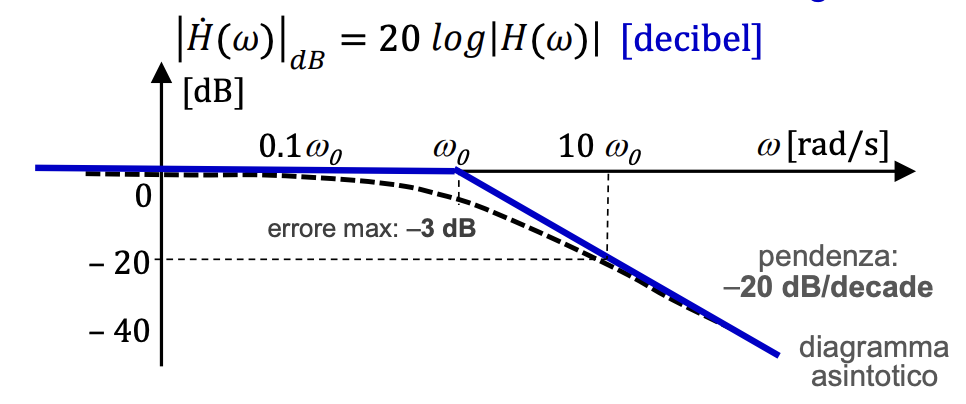
\includegraphics[scale=0.35]{immagini/pbbode}
	\caption{Modulo della risposta in frequenza in scala lineare e in scala logaritmica (diagramma di bode)}
\end{figure}
\newpage
\begin{figure}[h]
	\centering 
	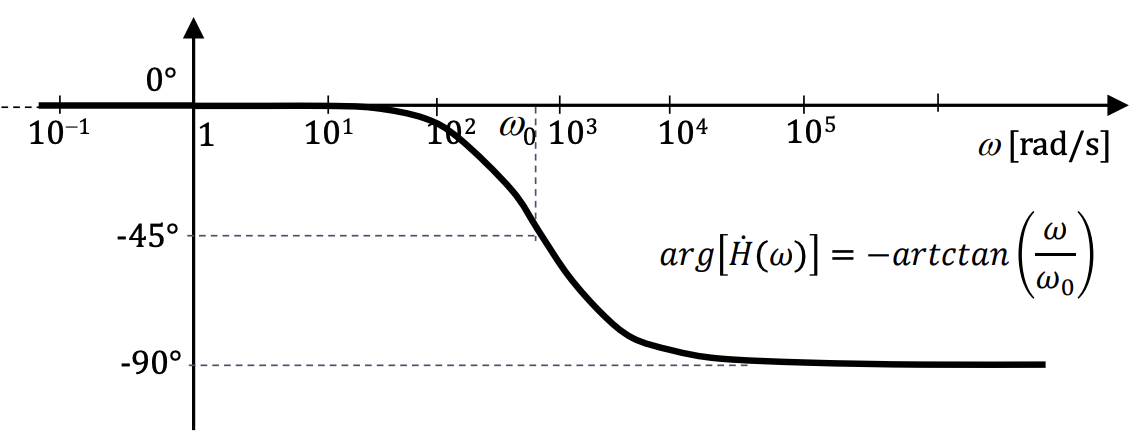
\includegraphics[scale=0.25]{immagini/pbg1}
	\hfil 
	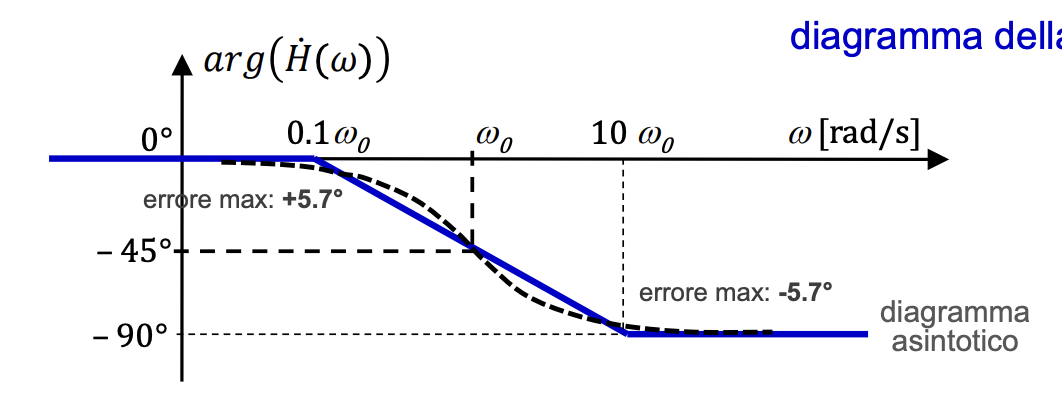
\includegraphics[scale=0.35]{immagini/pbbode1}
	\caption{Argomento della risposta in frequenza in scala lineare e in scala logaritmica (diagramma di bode)}
\end{figure}
\item \textbf{Filtro passo alto RC : }
\begin{center}
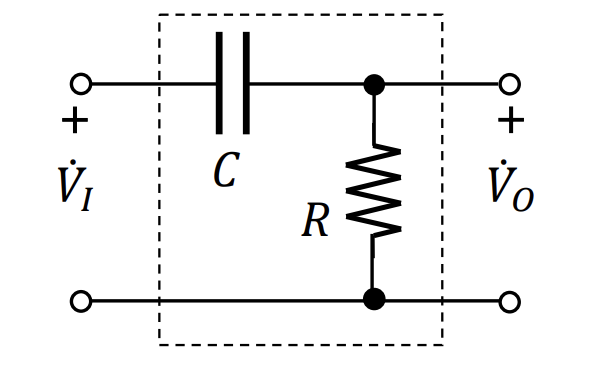
\includegraphics[scale=0.50]{immagini/pa}
\end{center}
\end{itemize}
Possiamo scrivere quindi la frequenza di risposta come 
$$H(\omega)=\frac{V_0(\omega)}{V_I(\omega)}=\frac{Z_2}{Z_1+Z_2}=\frac{R}{R+\frac{1}{j\omega C}}=
\frac{Rj\omega C}{Rj\omega C+1}=\frac{j\frac{\omega}{\omega_0}}{1+j\frac{\omega}{\omega_0}}\ \ \ \omega_0=\frac{1}{RC}$$
\begin{figure}[h]
	\centering 
	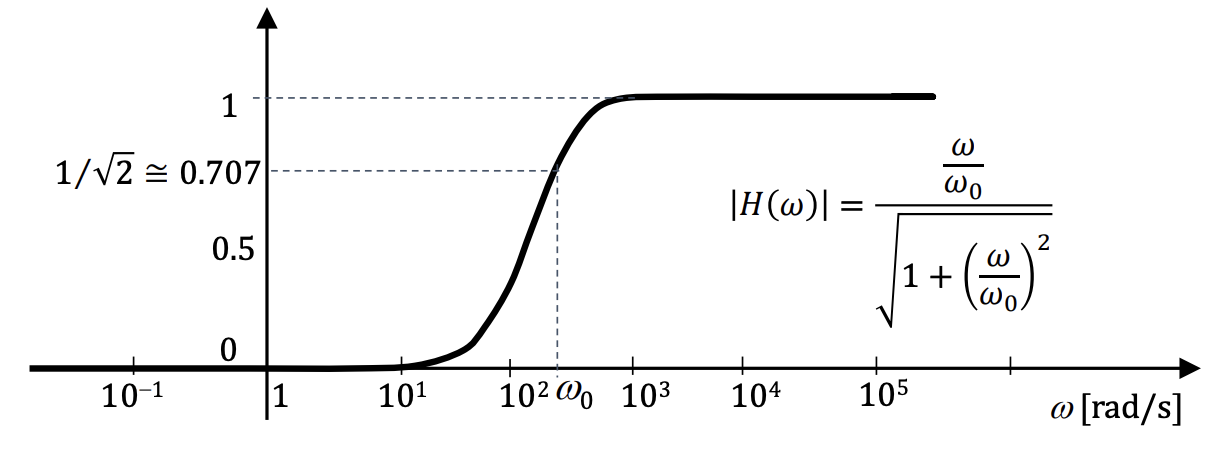
\includegraphics[scale=0.25]{immagini/pag}
	\hfil 
	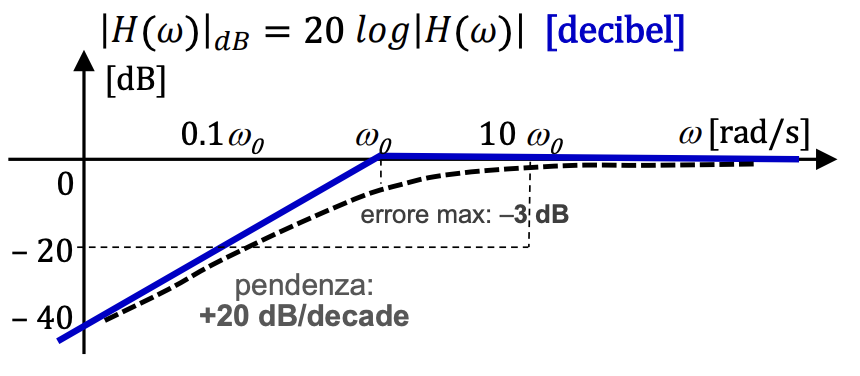
\includegraphics[scale=0.35]{immagini/pabode}
	\caption{Modulo della risposta in frequenza in scala lineare e in scala logaritmica (diagramma di bode)}
\end{figure}
\begin{figure}[h]
	\centering 
	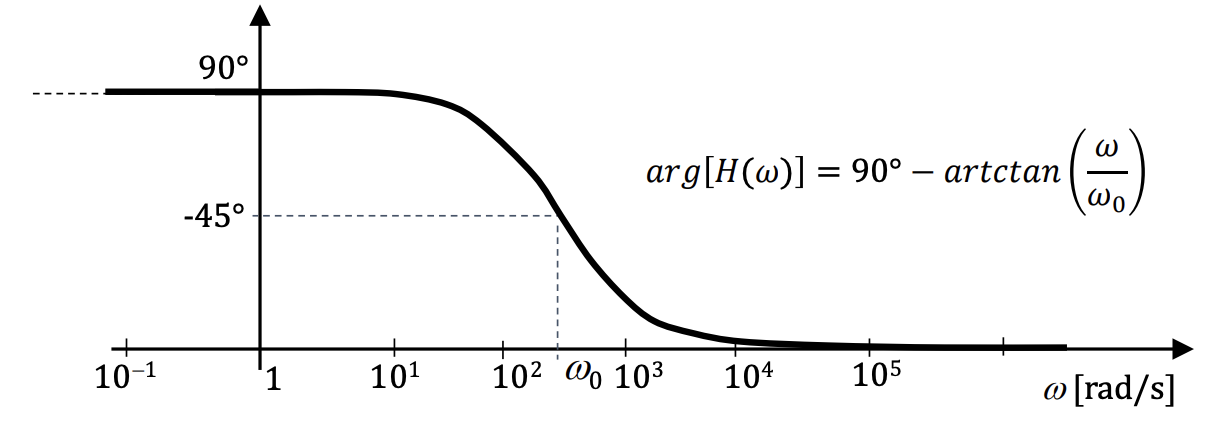
\includegraphics[scale=0.25]{immagini/pa1}
	\hfil 
	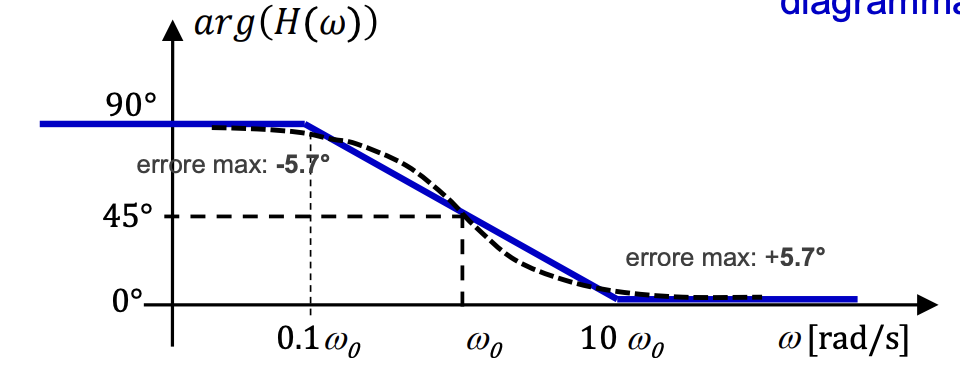
\includegraphics[scale=0.35]{immagini/pabode1}
	\caption{Modulo della risposta in frequenza in scala lineare e in scala logaritmica (diagramma di bode)}
\end{figure}
\item \textbf{Filtro RL passa basso: }
\begin{center}
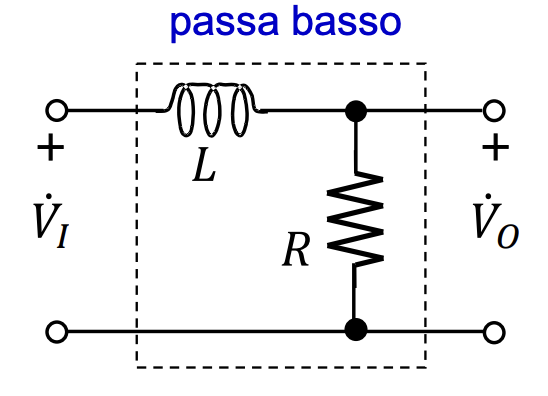
\includegraphics[scale=0.50]{immagini/pbl}
\end{center}
Possiamo ricavare la riposta in frequenza :
$$H(\omega)=\frac{V_0(\omega)}{V_I(\omega)}=\frac{Z_2}{Z_1+Z_2}=\frac{R}{R+jwL}=\frac{1}{1+j\frac{\omega}{\omega_0}} \ \ \ \omega_0=\frac{R}{L}$$
\item \textbf{Filtro passa alto RL:}
\begin{center}
	\includegraphics[scale=0.50]{immagini/pal}
\end{center}
$$H(\omega)=\frac{V_0(\omega)}{V_I(\omega)}=\frac{Z_2}{Z_1+Z_2}=\frac{jwL}{R+jwL}=\frac{j\frac{\omega}{\omega_0}}{1+j\frac{\omega}{\omega_0}} \ \ \ \omega_0=\frac{R}{L}$$
\end{itemize}
\paragraph{Cascata di filtri}
\begin{center}
\includegraphics[scale=0.40]{immagini/cascata}
\end{center}
	Quando due o più filtri sono collegati a cascata , l'uscita del primo filtro diventa l'ingresso del secondo , e così via.\\La risposta in frequenza complessiva sarà pari al prodotto di tutte le singole risposte in frequenza 
	$$H(\omega)=H_1(\omega)\cdot H_2(\omega) 	\cdot \dots\ \cdot \ H_n(\omega)$$
\paragraph{Filtro Passa Banda(con filtri del primo ordine)}
\begin{center}
\includegraphics[scale=0.60]{immagini/passa banda}
\end{center}
$$H(\omega)=\frac{V_0}{V_I}=\frac{V_0}{V}\cdot \frac{V}{V_1}=\frac{j\frac{\omega}{ \omega_1}}{1+j\frac{\omega}{\omega_1}}\cdot\frac{1}{1+j\frac{\omega}{\omega_2}}\ \ \ \ \omega_1=\frac{1}{R_1 C_1} \ \omega_2=\frac{1}{R_2C_2} \ \ \ \omega_1 <<\omega_2$$

\begin{figure}[h]
	\centering 
	\includegraphics[scale=0.35]{immagini/psb}
	\hfil 
	\includegraphics[scale=0.40]{immagini/psbode}
	\caption{Modulo della risposta in frequenza in scala lineare e in scala logaritmica (diagramma di bode)}
\end{figure}
\begin{figure}[h]
	\centering 
	\includegraphics[scale=0.35]{immagini/psb1}
	\hfil 
	\includegraphics[scale=0.35]{immagini/psbode1}
	\caption{Modulo della risposta in frequenza in scala lineare e in scala logaritmica (diagramma di bode)}
\end{figure}
\paragraph{Filtri di secondo ordine}
\begin{itemize}
	\item Filtro passa basso RLC:
	\begin{center}
\includegraphics[scale=0.50]{immagini/pbRLC}
$$H(\omega)=\frac{-jQ_s\frac{\omega_0}{\omega}}{1+jQ_s\left(\frac{\omega}{\omega_0}-\frac{\omega_0}{\omega}\right) }\ \ \ \ w_0)\frac{1}{\sqrt{LC}}$$
dove $Q_s=\frac{\omega_0 L}{R}$ è il fattore di qualità del circuito risonante
	\end{center}

\begin{figure}[h]
	\centering 
	\includegraphics[scale=0.35]{immagini/pbRLCg}
	\hfil 
	\includegraphics[scale=0.35]{immagini/pbRLCbode}
	\caption{Modulo della risposta in frequenza in scala lineare e in scala logaritmica (diagramma di bode)}
\end{figure}
\begin{figure}[h]
	\centering 
	\includegraphics[scale=0.50]{immagini/pbRLCg1}
	\caption{Modulo della risposta in frequenza in scala lineare}
\end{figure}
\item Filtro passa alto : \\
\begin{center}
\includegraphics[scale=0.50]{immagini/paRLC}
\end{center}
$$H(\omega)=\frac{jQ_s\frac{\omega}{\omega_0}}{1+jQ_s\left(\frac{\omega}{\omega_0}-\frac{\omega_0}{\omega}\right) }\ \ \ \ w_0)\frac{1}{\sqrt{LC}}$$
dove $Q_s=\frac{\omega_0 L}{R}$ è il fattore di qualità del circuito risonante

\begin{figure}[h]
	\centering 
	\includegraphics[scale=0.35]{immagini/paRLCg}
	\hfil 
	\includegraphics[scale=0.35]{immagini/paRLCbode}
	\caption{Modulo della risposta in frequenza in scala lineare e in scala logaritmica (diagramma di bode)}
\end{figure}
\begin{figure}[h]
	\centering 
	\includegraphics[scale=0.50]{immagini/paRLCg1}
	\caption{Modulo della risposta in frequenza in scala lineare}
\end{figure}
\item Filtro passa banda : 
\begin{center}
\includegraphics[scale=0.50]{immagini/passabRLC}
\end{center}
\begin{figure}[h]
	\centering 
	\includegraphics[scale=0.50]{immagini/passabg}
	\caption{Modulo della risposta in frequenza in scala lineare}
\end{figure}
$$H(\omega)=\frac{1                                                                                                                                                                                                  k}{1+jQ_s\left(\frac{\omega}{\omega_0}-\frac{\omega_0}{\omega}\right) }$$
La banda passante risulta centrata sulla pulsazione di risonanza $\omega_0$
\item FIitro elimina banda :
\begin{center}
\includegraphics[scale=0.40]{immagini/eliminabRLC}
\end{center}$$H(\omega)=\frac{jQ_s\left(\frac{\omega}{\omega_0}-\frac{\omega_0}{\omega}\right)}{1+jQ_s\left(\frac{\omega}{\omega_0}-\frac{\omega_0}{\omega}\right) } $$
\newpage
\begin{figure}[h]
	\centering
\includegraphics[scale=0.40]{immagini/eliminabg}
\caption{Modulo della frequenza di risposta}
\end{figure}

 \item Filtri passa banda realizza con una cascata di filtri
\begin{figure}[h]
	\centering
	\includegraphics[scale=0.35]{immagini/24}
	\includegraphics[scale=0.35]{immagini/25}
\end{figure}
\end{itemize}
\newpage
\section{Sistemi trifase}
Un sistema \textbf{polifase} è un'insieme di P tensione o correnti sinusoidali isofrequenziali. \\ Di conseguenza un sistema trifase è un sistema in cui sono presenti 3 tensioni o correnti isofrequenziali.
Inoltre un sistema trifase può essere :
\begin{itemize}
\item simmetrico;\\
Un sistema trifase è definito simmetrico se quando le sue tre fasi 
\begin{itemize}
	\item Hanno lo stesso valore efficace 
	\item Sono sfasate di $120^\circ$
\end{itemize}
\item diretto:\\
un sistema trifase è detto diretto quando quando le tre fasi rispettano l'ordine naturale di rotazione 
$$a(0^\circ)\rightarrow b (120^\circ)\rightarrow c(240^\circ)$$
\item puro:\\
un sistema trifase è pure quando la somma dei fasori (tensione o corrente) è pari a zero
\end{itemize}
\subsection{Collegamento a stella}
\subsubsection{Generatori}
\begin{figure}[h]
	\centering
	\includegraphics[scale=0.50]{immagini/stella}
	\label{fig:stella}
\end{figure}
Il nodo O è detto \textit{centro di stella}.\\Le tensioni stellate (di fase) tra fase e centro della stella coincidono con le tensioni dei generatori\\Le tensioni concatenate o di linea tra due fasi sono 
$$V_{12}=E_1-E_2 \ \ \ V_{23}=V_2-V_3 \ \ \ V_{31}=V_3-V_1 \ \ \ \text{Tutti i valori sono fasori}$$
inoltre nel caso di un sistema trifase diretto e simmetrico tutte le tensioni concatenate sono uguali e hanno valori efficaci pari a $$V=2E\cos{\frac{\pi}{6}}=\sqrt{3}E$$
\subsubsection{Utilizzatori}
\begin{figure}[h]
	\centering
	\includegraphics[scale=0.40]{"immagini/no neutro"}
	\label{fig:no-neutro}
\end{figure}
In questo caso le tre impedenze hanno valori diversi , quindi i tre carichi sono alimentati da una tensione diverse da quella dei generatori
$$V_{OO'}=\frac{\frac{\dot{E}_1}{\dot{Z}_1}+\frac{\dot{E}_2}{\dot{Z}_2}+\frac{\dot{E}_3}{\dot{Z}_3} }{\frac{1}{\dot{Z}_1}+\frac{1}{\dot{Z}_2}+\frac{1}{\dot{Z_3}}} \ \ \ \ \dot{I}_K=\frac{\dot{E}_K-V_{OO'}}{\dot{Z}_K}$$
\newpage
Per poter alimentari i carichi usando le tensione dei generatori viene introdotto un quarto filo chiamato neutro che collega O' a O 
\begin{figure}[h]
    \centering
    \includegraphics[scale=0.40]{immagini/neutro.png}
    \label{fig:enter-label}
\end{figure}
In questo caso le correnti di linea hanno espressioni $\dot{I}_K=\frac{\dot{E}_K}{\dot{Z}_K}$ e la corrente nel neutro è pari a $I_O=I_1+I_2+I_3$ (fasori).\\
Se prendiamo in esame un sistema trifase simmetrico e con carico equilibrato , le impedenza dei carichi sono uguali tra loro) allora abbiamo due risultati interessanti:
\begin{itemize}
    \item $\dot{V}_{OO'}=0$ poichè i due centri sono collegati dal neutro
    \item La terna delle tre correnti è anch'essa simmetrica , sfasata solo di un angolo $\phi=arg(\dot{Z})$ rispetto alla terna delle tensioni
    \begin{center}
        \includegraphics[scale=0.20]{immagini/phi.png}
    \end{center}
    \item $I_0=0$ per cui il neutro può essere eliminato
\end{itemize}
\subsection{Collegamento a triangolo}
\subsubsection{utilizzatori}
\begin{figure}[h]
    \centering
    \includegraphics[scale=0.30]{immagini/t1.png}
    \hfil
    \includegraphics[scale=0.30]{immagini/t2.png}
\end{figure}
Le correnti di fase che scorrono nelle impedenze sono pari a 
$$\dot{J}_{ik}=\frac{\dot{V}_{ik}}{\dot{Z}_{ik}}$$
$$\dot{I}_1=\dot{J}_{12}-\dot{J}_{31} \ \ \ \dot{I}_2=\dot{J}_{23}-\dot{J}_{12} \ \ \ \dot{I}_3=\dot{J}_{31}-\dot{J}_{23}$$
Se abbiamo un sistema di generatori simmetrico ed un carico equilibrato hanno le correnti di fase hanno lo stesso valore efficace 
$$I=2J\cos{\frac{\pi}{6}}=\sqrt{3}J$$
\begin{figure}[h]
    \centering
    \includegraphics[scale=0.45]{immagini/1234.png}
  
    \label{fig:enter-label}
\end{figure}
\subsection{Potenza in sistemi trifase}
Potenza istantanea fornita dal tripolo :
$$p(t)=e_1(t)_1(t)+e_2(t)i_2(t)+e_3(t)i_3(t) $$
Potenza complessa fornita dal tripolo:
$$\dot{S}=\dot{E}_1\dot{I}_1^*+\dot{E}_2\dot{I}_2^*+\dot{E}_3\dot{I}_3^*$$ inoltre possiamo dimostrare che la potenza complessa e la potenza istantanea non dipendono dal riferimento dei potenziali.
Quindi ora possiamo calcolare :
\begin{itemize}
    \item potenza attiva trifase:
$$P=Re[\dot{S}]=E_1I_1\cos{\phi_1}+E_2I_2\cos{\phi_2}+E_3I_3\cos{\phi_3}$$
    \item potenza reattiva trifase
    $$Q=Im[\dot{S}]=E_1I_1\sin{\phi_1}+E_2I_2\sin{\phi_2}+E_3I_3\sin{\phi_3}$$
\end{itemize}
Una sezione di linea trifase simmetrica , ed equilibrati ( quindi le Tensione e le correnti sono sfasate di 120 gradi) abbiamo che la potenza istantanea è pari a:
$$p(t)=e_1(t)_1(t)+e_2(t)i_2(t)+e_3(t)i_3(t)=3EI\cos(\phi)$$
Quindi nella sezione vediamo che la potenza istantanea è costante ed è parti alla potenza attiva , quindi NELLA sezione la potenzia reattiva è pari a zero ( fluttua invece nelle singole linee).
Utilizzando le grandezza di linea possiamo scrivere 
$$p(t)=P=\sqrt{3}VI\cos{\phi} \ \ \ \ Q=\sqrt{3}VI\sin{\phi}\ \ \ \ S=\sqrt{3}VI$$
\subsection{Misure in sistemi trifase}
\begin{itemize}
    \item corrente: Ne dobbiamo usare 3 0 4(neutro) se invece il sistema è equilibrato ne basta 1 amperometro
    \item tensione: dobbiamo usare 3 voltmetri , se il sistema è simmetrico basta 1 voltmetro 
    \item Potenza: 
   \begin{itemize}
       \item  In sistemi con neutro vanno usati 3 wattmetri , se il sistemi è simmetrico ed equilibrato basta 1 wattmetro
       \item In sistemi senza neutro vanno usati 2 wattmetri (\textbf{inserzione Aron}) una fase è considerata linea di ritorno delle altre due fasi della potenza misurata dipende da polarità dai morsetti amperometrici e voltmetrici , inoltre non sono richiesta ipotesi su tensioni e correnti 
       $$P=P_{13}+P_{23}$$
   \end{itemize}
\end{itemize}











\end{document}

